\documentclass[journal,final]{new-aiaa}
\usepackage[utf8]{inputenc}
\usepackage{color}
\usepackage{algorithm}
\usepackage[noend]{algpseudocode}
\usepackage{graphicx}
\usepackage{amsmath}
\usepackage[version=4]{mhchem}
\usepackage{siunitx}
\usepackage{longtable,tabularx}
\setlength\LTleft{0pt}

\newcommand{\A}{\mathbf{A}}
\newcommand{\B}{\mathbf{B}}
\newcommand{\C}{\mathbf{C}}
\newcommand{\D}{\mathbf{D}}
\newcommand{\E}{\mathbf{E}}
\newcommand{\F}{\mathbf{F}}
\newcommand{\G}{\mathbf{G}}
\newcommand{\HH}{\mathbf{H}}
\newcommand{\I}{\mathbf{I}}
\newcommand{\J}{\mathbf{J}}
\newcommand{\K}{\mathbf{K}}
\newcommand{\LL}{\mathbf{L}}
\newcommand{\PP}{\mathbf{P}}
\newcommand{\R}{\mathbf{R}}
\newcommand{\U}{\mathbf{U}}
\newcommand{\W}{\mathbf{W}}
\newcommand{\w}{\mathbf{w}}

\newcommand{\uu}{\mathbf{u}}
\newcommand{\n}{\mathbf{n}}
\newcommand{\rr}{\mathbf{r}}
\newcommand{\s}{\mathbf{s}}
\newcommand{\e}{\mathbf{e}}
\newcommand{\ddd}{\mathbf{d}}
\newcommand{\f}{\mathbf{f}}
\newcommand{\T}{\mathbf{T}}
\newcommand{\x}{\mathbf{x}}
\newcommand{\y}{\mathbf{y}}
\newcommand{\ttt}{\mathbf{t}}
\newcommand{\bb}{\mathbf{b}}

\newcommand{\vv}{\mathbf{v}}
\newcommand{\boldalpha}{\boldsymbol{\alpha}}


\newcommand{\df}[2]{\dfrac{\partial#1}{\partial#2}}
%\newcommand{\dd}[3]{\dfrac{\partial^2#1}{\partial#2 \partial#3}}
\newcommand{\dd}[3]{{\partial^2#1}/{\partial#2 \partial#3}}
\newcommand{\ff}[2]{\dfrac{d#1}{d#2}}
\newcommand{\ds}[2]{\dfrac{\partial^2#1}{\partial#2^2}}
\newcommand{\dn}[3]{\dfrac{\partial^{#1}#2}{\partial#2^{#1}}}

\newcommand{\dis}{\displaystyle}

\newcommand{\npo}{n\!\!+\!\!1}

\newcommand{\grad}{\textrm{grad\,}}
\newcommand{\Div}{\textrm{div\,}}

\newcommand{\half}{\frac{1}{2}}
\newcommand{\third}{\frac{1}{3}}
\newcommand{\quarter}{\frac{1}{4}}

\newcommand{\Atv}{\A^{\!T}\!v}
\newcommand{\Au}{\A u}
\newcommand{\RK}{R-K\@\xspace}
\newcommand{\vtf}{v^T\!f}
\newcommand{\gtu}{g^T\!u}

\newcommand{\degr}{^{\circ}}
\newcommand{\logt}{\log_{10}}
\newcommand{\dsps}{\displaystyle\strut}

\newcommand{\ind}{\phantom{\bf do}}

\graphicspath{{./pic/}}

\title{Flow instability prediction via eigenanalysis and its application to rotating stall}
\author[1,2]{Shenren Xu	
\footnote{Associate Professor, School of Power and Engery; shenren\_xu@nwpu.edu.cn}}
%\footnote{ Corresponding author, email address: shenren\_xu@nwpu.edu.cn}


\affil[1]{Yangtze River Delta Research Institute of NPU, Northwestern Polytechnical University, Taicang~215400, P.R.~China}

\affil[2]{Northwestern Polytechnical University, Xi'an 710072, P.R.~China}
\affil[3]{Beihang University, Beijing 100191, P.R.~China}
\author[3]{Chen He\footnote{Ph.D. Candidate, School of Energy and Power Engineering; hechen@
		buaa.edu.cn (Corresponding Author) }}
\author[3]{Dakun Sun\footnote{Associate Professor, School of Energy and Power Engineering; Co-Innovation
		Center for Advanced Aero-Engine; sundk@buaa.edu.cn}}
%\author[3]{Xiaofeng Sun\footnote{Professor, School of Energy and Power Engineering; Co-Innovation Center for Advanced Aero-Engine; sunxf@buaa.edu.cn}}
\author[2]{Dingxi Wang\footnote{Professor, School of Power and Engery; dingxi\_wang@nwpu.edu.cn }}

\begin{document}
\maketitle

\begin{abstract}
Global linear stability analysis is an effective way to predict the exact condition
at which flow goes unstable. Compared to the time-domain simulation approach,
eigenanalysis method can equivalently predict the destabilization
condition, but at a much lower cost, since unsteady simulations are no longer required.
In this work, a Newton--Krylov nonlinear flow solver is used to first solve for the
steady state flow solution and then eigenanalysis is performed by applying the 
implicit-restart Arnoldi method to the exact Jacobian matrix.
By tracking a subset of the eigenspectrum that is close to the imaginary axis,
the least stable eigenmodes can be found. By perturbing the bifurcation parameter,
e.g., the Reynolds number, the Hopf bifurcation point can be identified.
This method is applied to find the critical Reynolds number for a laminar
flow around a circular cylinder above which laminar vortex shedding appears.
Time-accurate unsteady simulation confirms the correctness of the critical eigenvalue
and eigenvector found. It is also applied to a quasi-3D compressor rotor
annular cascade case, for which eigenanalysis is performed and flow physics
is analyzed based on the unstable modes identified. Interesting correlation
between the rotating perturbation pattern and cell rotating speed is found,
which resembles what is observed in experiments.
This work is a first step towards the study of
rotating flow instabilities turbomachines, such as rotating stall and rotating instability,
and the preliminery results proved promising for future
application to three-dimensional practical problems.
	
	
%The compression system in turbomachines, e.g.,  aircraft engines and gas turbines,
%when operating under off-design conditions, exhibits self-excited unsteady phenomena
%such as surge, rotating stall and rotating instability, leading to performance deterioration
%and/or structural damages. Inability to accurately predict when such flow instability occurs
%limits the development of high performance compression system.
%Conventional methods for predicting the onset of such instabilities include analytical,
%semi-analytical-semi-empherical, and unsteady computational fluid dynamics (CFD) simulation,
%which are either fast but less accurate, or more accurate but requires long computational time.
%For engineering application, only steady state CFD analyses are affordable for deployment
%in practicla workflow. 
%In this paper, we explore using the eigenanalysis approach to predict the onset of such
%instabilities. The key benifit of such analysis is that it is capable to capture exactly the
%eigenmodes that destabilize with computational cost of a few steady analyses.
%Pivotal to such analysis is a robust steady state RANS flow solver using the Newton--Krylov
%time-integration scheme which explicitly forms the Jacobian matrix. Once the flow has
%converged fully, the Jacobian matrix is used to compute the relavent eigenvalues and vectors.
%The methodology is applied to the computation of stability boundary of
%(i) the laminar flow around a two-dimensional circular cylinder, and
%(ii) the flow around a quasi-three-dimensional compressor anuular cascade.
%The method developed here has the potential to revive the once-popular
%eigenvalue method for prediction rotating stall and surge, and to provide
%industry with tools to accurately predict the stall line in the early design stage.
\end{abstract}

%\section*{Nomenclature}
%{\renewcommand\arraystretch{1.0}
%\noindent\begin{longtable*}{@{}l @{\quad=\quad} l@{}}
%$c_v,c_p$   & specific heat \\
%$e$     & internal energy\\
%$E$     & total energy\\
%
%$\partial \Omega_r$& boundary of $\Omega_r$
%\end{longtable*}}

%{\Large \color{red} Tasks}
%
%\begin{enumerate}
%	\item{\color{red} finalize gpps paper}
%	\item  {\color{red} Literature review for rotating stall:}
%	\begin{enumerate}
%		\item {\color{red} M-G theory?}
%		\item {\color{red} Subsonic, how many cells? when? roating speed?}	
%		\item {\color{red} Transonic, how many cells? when? rotating speed?}
%		\item {\color{red} Active control achievement so far? low or high speed?}
%		\item{\color{red} Shortcoming of existing theory and applications?}				
%	\end{enumerate}
%\item  {\color{red} high speed steady performance curve? mesh convergence? validation?
%spectrum? find all ND=1-11? or even 12-22? how to explain 5+17=22?}
%\item{\color{red} same conclusion for low speed? same conclusions?}
%\item{\color{red} urans for confirmimg the eigenanalysis?}
%
%\end{enumerate}


\section{Introduction}
Rotating stall and rotating instability have been studied extensively
both experimentally~\cite{emmons1955compressor,frank1955propagation,emmons1959survey}
and numerically~\cite{cornelius2014experimental,he1997computational,vo2008control,pullan2015origins}.
Early experimental work revealed
the basic features of such phenemenon and subsequent work has focused
on building simple analytical models.
Existing analytical models~\cite{emmons1955compressor,greitzer1986theory} have
had their success in the early days but the accuracy and effectiveness of them
is less than sastifactory when applied to realistic configurations and
more details are needed for quantitative prediction of the stall behavior.

Previous numerical investigations mainly focused on using time-dependent
unsteady flow analysis using either a fraction or the whole of an annulus.
A lot of insight into the flow physics for the destablization mechanism
has been gained using such high fidelity simuations. Unsteady simulations
are useful for both reproducing the fully destabilized unsteady flows as
well as for studying the inception of such instability. Due to the high
computatioal cost of unsteady simulation, it still remains largely as a
reserach tool to investigate the stall phenomenon on a case-by-case
basis.

It is widely believed that the fully developed stall and surge behavior is quite
different from the incipient stall, or pre-stall disturbance~\cite{stenning1980rotating},
as fully developed rotating stall exhibits strong nonlinearity. However, if the goal is
to apply active control to suppress the instability at its infancy, then a linear stability
prediction should suffice, as has been demonstrated in numerous work~\cite{paduano1991active,day1993active,paduano2001compression,day1997stall},
as the idea is to eliminate the fully-developed rotating cells from forming.

As modern compression systems are designed with higher loading and speed,
most analytical models proposed in the early days and desmontrated useful
on low-speed machines are no longer useful as compressibility and complex
flow mechanism such as boundary-layer-shock-wave interaction becomes
important. In addition, existing models seldom take into account the exact
geometry of the blading, and instead, a simple correlation of the compressor
characteristics is used. This is obviously not desirable as
geometry details, such as the exact leading geometry, have great impact
on the stall characteristics. This is particularly the case when more complex stall
phenomenon are considered, such as spike stall, where geometry details
such as tip gap and the leading edge shape play a major role.

This calls for a stability analysis method based on the three-dimensional
Reynolds-averaged Navier-Stokes equations, which is regarded as
the standard industrial tool for predicting steady and unsteady turbomachinery
performance. In a way, existing stall model needs to be upgraded using the latest
high-fidelity flow models. Again, either time-dependent simulations or
steady-state-based eigenanalysis can be used to study the stability based
on the high-fidelity models and each has its strength. Time-dependent
analysis is able to capture not only the incipent stall behavior but also the
details of the transient process, but with a very high computational cost.
Eigenvalue analysis is a powerful yet inexpensive tool to probe the flow
near the critical condition, but is still capable of revealing rich flow physics,
with cost comparable to a few steady state analysis.

In this work, we demonstrate that using eigenanalysis based on a whole-annulus
steady state solution, the linear stablity demarcation point can be pinpointed
with the cost of a few steady state analysis, and a full-annulus time-accurate
unsteady calculation can thus be avoid. This methodology enables quick parameter
study to investigate the various rotating flow instability phenomenon
such as rotating stall and rotating instability.

The idea is performing such eigenanalysis is simple. The difficulty is in the detail.
One common misunderstanding is that an eigenanalysis for large cases is expensive.
This is true only if we were to compute the full spectrum of a large sparse linear system
using direct method~\cite{amestoy2000mumps}.
However, since a subset of the millions or even billions of eigenvalues are relevant regarding
the linear stability, typically $\mathcal O(100)$, such eigenanalysis can be done at the cost of
a few steady state analysis, using iterative eigenvalue calculation
methods~\cite{sorensen1992implicit,lehoucq1998arpack}.

In practics, such eigenanalysis is rarely done for large, complex cases of industry relevance.
The challenge is twofold. First,
in order to perform eigenanalysis, a steady state flow solution should first be
obtained, requiring the full convergence of the flow solver. While this is easily
achievable at design condition, obtaining a fully converged solution for off-design
conditions remains a challange from the perspective of flow solver~\cite{xu2015stabilisation}.
This is seldom discussed in literature, but widely felt in industry. Secondly, it is
a common belief such the computatinal cost of such eigenanlysis is overwhelming
and is thus impractical for real application. With the maturing of distributed
computing, this is no longer the bottleneck and one can easily compute the
relevant eigenvectors for cases with up to 10 million grid point, and the cost
only increases linearly with a scalable algorithm. But here the focus shifts slightly
to the computational methods side from the flow physics . But as discussed
in~\cite{day2016stall}, combinging the advancement by computational specialists
and the expertise from the `stall fraternity' is the right way to advance the research
in compressor stall study and an effective way to harness better the benifit of
using CFD. In this paper, we attempt to apply the latest development in large
scale eigenanalysis computational method to the long-standing problem of
rotating flow instability, rotating stall in particular, and try to explore the
underlying flow physics governing the pre- and in-stall behavior, with a
computational cost that is affordable for industrial applications.

The rest of this paper is organized as follows. First, the basic algorithm of the
nonlinear flow solver will be discussed in sec.~\ref{lable:sec1}. Fundemantals of 
performing eigenanalysis based on RANS equations and relevant techniques
are discussed in sec.~\ref{label:sec2}. Results for the application of eigenanalysis
to predict flow instability is elaborated in sec.~\ref{label:results} and conclusions
are drawn in sec.~\ref{conclusion}.



\section{The nonlinear flow solver}
\label{lable:sec1}
The nonlinear flow solver used in this work is NutsCFD, an unstructured-mesh
finite-volume RANS solver capable of dealing with rotating frame reference
and periodic boundary conditions.
The solver features the use of the Newton--Krylov algorithm,
which significantly enhances the efficiency and robsutness when
computing turbomachinery flows at off-design conditions.
Details of the solver can be found in~\cite{xu2019nk}
and a brief description of the solution algorithm is provided in this section.

\subsection{Governing equations}
The integral form of the governing equations in a
relative frame of reference with a constant angular
velocity of $\boldsymbol \omega$ is
\begin{equation*}
\dfrac{d}{dt}\int_{\Omega_r} \W dV
+\oint_{\partial \Omega_r} (\F^r_c-\F_v)dS
+\int_{\Omega_r}\F_\omega dS
=0,
\label{governing}
\end{equation*}
where $\W$ are %is
the conservative variables
$\left[\rho,~\rho\uu,~\rho E\right]^T$.
The absolute and relative convective fluxes,
$\F_c$ and $\F^r_c$,
the viscous flux $\F_v$,
and the additional flux due
to rotation, $\F_\omega$,
are defined as %follows
\begin{equation*}
\F_c=
\left [ 
\begin{array}{c}
\rho \uu \cdot \n\\
\rho \uu \uu\cdot \n +  p\n\\
\rho H \uu \cdot \n
\end{array}
\right],
\text{~~}
\F^r_c=
\F_c
-
(\uu_{rot}\cdot \n) 
\left [ 
\begin{array}{c}
\rho\\
\rho \uu\\
\rho E
\end{array}
\right ]
,\text{~~}
\F_v=
\left [ 
\begin{array}{c}
0\\
\tau \cdot \n\\
\uu \cdot \tau \cdot \n + \kappa \n \cdot \nabla T
\end{array}
\right ],\text{~~}
\F_\omega=
\left [ 
\begin{array}{c}
0\\
\rho {\boldsymbol{\omega}} \times \uu\\
0
\end{array}
\right ],
\end{equation*}
with $\uu_{rot}={\boldsymbol \omega} \times \x$.
When $\omega$ is zero, a solver applicable to
non-rotating reference frame is recovered.

Flow is assumed to be fully turbulent and turbulence is
modeled using the negative Spalart--Allmaras
(SA-neg) model~\cite{allmaras2012modifications}.
Compared to the original SA model~\cite{spalart1992one},
this avoids the clipping of the turbulent variable
to a non-negative value which potentially
prevents the full convergence of the nonlinear solver.
The turbulence equation is discretized using
the first-order accurate upwind
scheme~\cite{langer2014agglomeration}.

\subsection{Spatial discretization}
The governing equations are discretized using the
method of lines and thus the spatial and temporal
discretizations can be treated separately.
The governing equations for
the
steady-state solution $\W$
is
\begin{equation}
\label{nonlinear}
\R(\W)={\bf 0},
\end{equation}
where $\R$ is the sum of fluxes and source terms
associated with each control volume. Suppose control
volume %node
$i$ has $N$ flux faces with
area $S_{ik}$ for
$k=1,2,...,N$.
$R_i$ then is 
\begin{equation*}
R_i(\W)=\sum^{N}_{k=1} (\F^r_c-\F_v)S_{ik}+\F_{\omega} V_i,
\end{equation*}
where $V_i$ denotes the volume.
The computation of the convective flux $\F^r_c$ is based on a modification
of the Roe flux scheme to account for the relative reference
frame that is rotating with a constant angular velocity;
while the viscous flux $\F_v$ is the same as in the stationary
reference frame.



\subsection{Temporal discretization}
The Newton method solves the steady-state nonlinear
equation~\eqref{nonlinear} iteratively as %follows
\begin{equation*}
\W^{n+1}=\W^n+\beta \Delta \W
\label{newtonTransient}
\end{equation*}
until convergence is reached, i.e., $\|\R(\W)\|=0$,
where $\Delta \W$ is the solution to the linear 
system of equations
\begin{equation*}
\df{\R}{\W}\Delta \W = -\R(\W^n),
\end{equation*}
while $\beta$ is an under-relaxation factor 
obtained using a line search.

Once the spatial discretization,  $\R(\W^n)$, is established,
there are three main steps to complete a Newton update step,
namely, (i) forming the Jacobian matrix, (ii)
solving the large sparse linear system of equations,
and (iii) finding a step size $\beta$ and update the nonlinear
flow solution.
To form the Jacobian matrix, automatic differentiatino tool Tapenade~\cite{Tapenade}
is used, together with graph coloring tool Colpack~\cite{gebremedhin2013colpack}.
By executing the
foward-differentiated residual subroutine for a subsets of nodes
with the same color, the Jacobian matrix is calculated. The resulting
large sparse linear system of equations is solved using GMRES
right-preconditioned by the incomplete LU factorization with zero
fill-in. 



\section{Global linear stability analysis via eigenmode decomposition}
\label{label:sec2}
\subsection{Global linear stability analysis}
A nonlinear dynamic system, e.g., the discretised NS equation discretized
using the method of lines,
has the form
\begin{equation*}
Vol \dfrac{d\uu}{dt}=-\R(\uu)
\end{equation*}
where $\uu$ is the time-varying flow variable and $\R(\uu)$ is the nonlinear
residual representating the spatial discretization.
$Vol$ is a diagonal matrix with the volume of each dual cell on its diagonal.
This term can be eliminated by redefining $\R(\uu)$ by applying volume
scaling to it. The governing equation of the dynamic system then becomes
\begin{equation*}
\dfrac{d\uu}{dt}=-\R(\uu)
\end{equation*}

Assuming a steady state solution $\uu_0$ (equilibrium point of the dynamic system)
exists, and the time-varying flwo variable can be decomposed as the
steady and the unsteady part 
\begin{equation*}
\uu:=\uu_0 + \tilde \uu
\end{equation*}
and the governing equation becomes
\begin{equation*}
\dfrac{d \tilde \uu}{dt}=A \tilde \uu
\end{equation*}
where $A$ is the negative Jacobian $A:=-\df{\R}{\uu}$.

In order to use the eigen model decomposition approach, suppose
the system matrix has right eigenvectors $\{\vv_i, \vv_2, ..., \vv_N\}$,
which forms the matrix $V$ as its colum vectors. Matrix $A$ can then
be factorized as 
\begin{equation*}
A=V\Lambda V^{-1}
\end{equation*}
where the diagonal matrix $\Lambda$ has the eigenvalues of the matrix $A$
as its diagonal elements.
Decomposing the unsteady part $\tilde \uu$ in the eigen modal space with
coordinates $\eta$
\begin{equation*}
\tilde \uu = V {\mathbf \eta}.
\end{equation*}
Substituting $\tilde \uu$ in the governing equation using the eigen modal
decomposition, it becomes
\begin{equation*}
\dfrac{d \eta}{dt}= \Lambda \eta.
\end{equation*}
All equations are decoupled now and can be written as
\begin{equation*}
\dfrac{d \eta_i}{dt}= \lambda_i \eta_i  ~~~\forall i.
\end{equation*}
For the linear system to be stable, a sufficient condition is
that all eigenvalues have negative real parts, i.e., real$(\lambda_i)<0, \forall i$.

\subsection{Numerical implementation of eigenanalysis}
In theory, performing the global linear stability analysis as described above
is a standard procedure involving three steps: (i) find an equilirium point $\uu_0$;
(ii) linearize the nonlinear residual and form the Jacobian matrix $A$, and
(iii) perform eigenanalysis and find $\Lambda$ and $V$. Step (i) is simply
running the steady state flow solver until a steady state solution
is found. Step (ii) is a by-product of the nonlinear flow calculation using
the NK method, i.e., store away the Jacobian matrix at the final Newton step.
Step (iii) is a bit more involved for high dimensional problems.

For eigenmode computations, the implicitly restarted Arnoldi method proposed
by Sorensen~\cite{sorensen1992implicit} and implemented in the ARPACK
library~\cite{lehoucq1998arpack}, is used
in combination with the NutsCFD solver.
Shift-and-invert spectral transformation is applied to converge to wanted parts
of the eigenspectrum, and critical is therefore the robust solution of many linear
systems of equations. 
Key to efficiently solving the arising large sparse linear system of equations
is the deflated Krylov subspace solver GCRO-DR~\cite{parks2006recycling}.
Compared with the more commonly used GMRES solver~\cite{saad1986gmres},
GCRO-DR is both more CPU time and memory efficient, especially as the system
matrix condition worsens, as demonstrated in~\cite{xu2016enabling,xu2017robust}.

\section{Results}
\label{label:results}

\subsection{Laminar flow around a two-dimensional circular cylinder}
Eigenvalue analysis is performed for the canonical case of the
laminar flow around a circular cylinder with the Reynolds number in
the range between 40 and 100. The computational domain is a
circular cylinder centered at the origin with a diameter of $D=10^{-5}$
and the farfield is a circle with a diameter of $100D$. The left half of
the outer circle is set to 'farfield' boundary condition with a incoming
flow of Mach 0.2 in the x-direction, a static pressure of $101325~Pa$ and
and a temperature of $288.15~K$.
The right half ot he circle is set to 'pressure-outlet' boundary condition,
with a constant pressure of $101325~Pa$.
The computational domain is meshed with quadrilateral elements,
with a total of 29600 grid points. The density is $1.225~kg/m^3$.
The dynamic viscosity is varied in order to achieve a particular Reynolds number.

\subsubsection{Steady state calculation}
The steady state flow solution for $Re=55$ is obtained by either using an implicit solution method in
Fluent (version 19.2) or by resorting to the Newton-Krylov algorithm in NutsCFD,
despite the fact that the flow is physically unsteady under this condition. The
Mach number contour of the NutsCFD calculation is shown in Fig.~\ref{fig:cyl-re55}.

\begin{figure}[htb]
	\centering   
	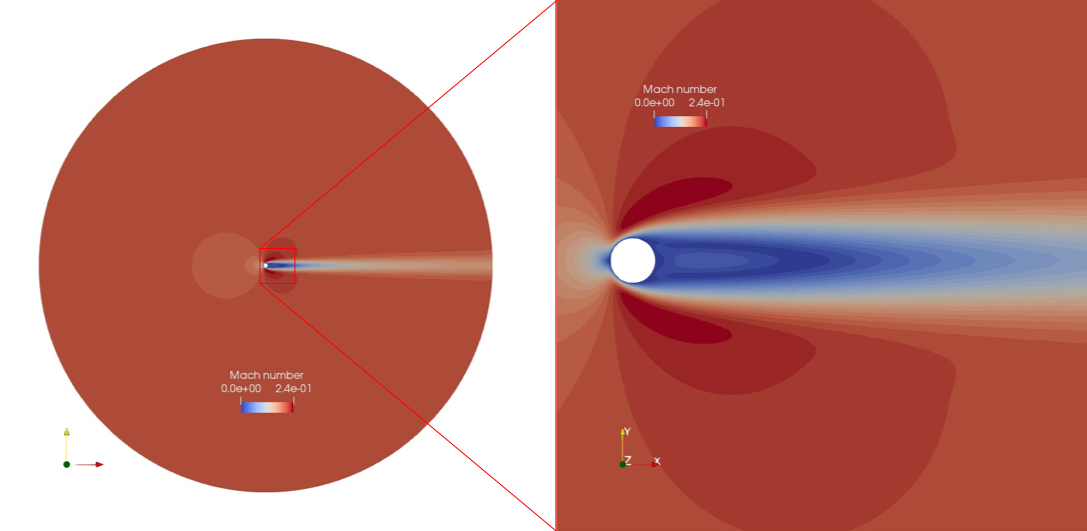
\includegraphics[width=0.5\textwidth]{pic/cylinder-std.png}
	\caption{Mach number contour plot of the calculation results by NutsCFD for $Re=55$.}
	\label{fig:cyl-re55}
\end{figure}

To compare the Fluent and NutsCFD results quantitatively, the x-velocity
behind the cylinder and the pressure coefficient along the cylinder
surface are compared in Fig.~\ref{fig:cyl-re55-u-cp} and very good agreement
can be found.
\begin{figure}[htb]
	\centering   
	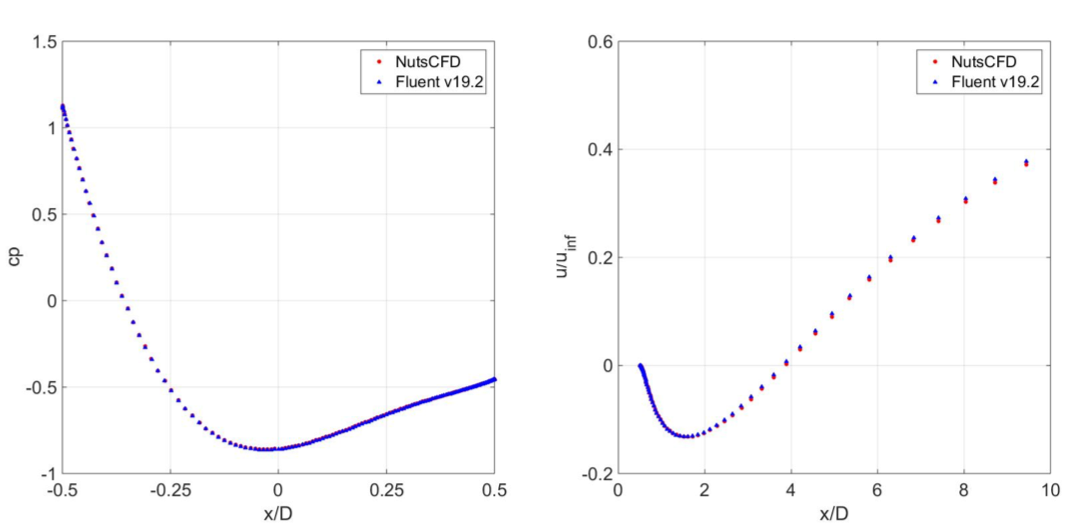
\includegraphics[width=0.5\textwidth]{pic/cylinder-std-compare.png}
	\caption{Comparison between Fluent and NutsCFD calculation results for
		x-velocity along the center line behind the cylinder (left) and pressure
		coefficient along the cylinder surface (right).}
		\label{fig:cyl-re55-u-cp}
\end{figure}

\subsubsection{Unsteady calculation}
Experimental results show that the laminar flow around the cylinder
becomes unsteady for Re above a critical value (around 47). To study
this phenomenon, unsteady flows for $Re=55$ and $Re=40$
are performed using NutsCFD. First, for both conditions, a steady
state flow solution is obtained by converged the residual to machine error.
Then, unsteady simulation is run with the steady state
as initial condition for $Re=55$.
A BDF2 second-order implicit dual-time-stepping
method is used with the physical time step set to
$10^{-8} sec$, that is, $0.01 ms$, and
the inner loop is solved with a maximum of 3 Newton iterations.
From Fig.~\ref{fig:cyl-re40-re55-uns}, it can be seen
that after around $100 ms$, the lift coefficient starts to grow and
eventually reaches a saturated limit cycle at around $130 ms$.
On the contrary, running unsteady simulation with a fully converged
steady state for $Re=40$ does not lead to unsteadiness. To probe
the flow at $Re=40$ further, a disturbance is introduced into the
flow from the farfield by setting the incoming flow direction to vertical
for one time step and switching it back to the x-direction,
and then continue the unsteady run. The lift coefficient shows a
transient growth but eventually slowly delays to zero. The
two sets of lift coefficient signals for $Re=40$ and $Re=55$
are plotted in Fig.~\ref{fig:cyl-re40-re55-uns}
in both linear and logrithm scales. The logrithmic plot on the right
clearly shows an exponential growth/decay for $Re=55$ and $Re=40$,
respectively.

\begin{figure}[htb]
	\centering   
	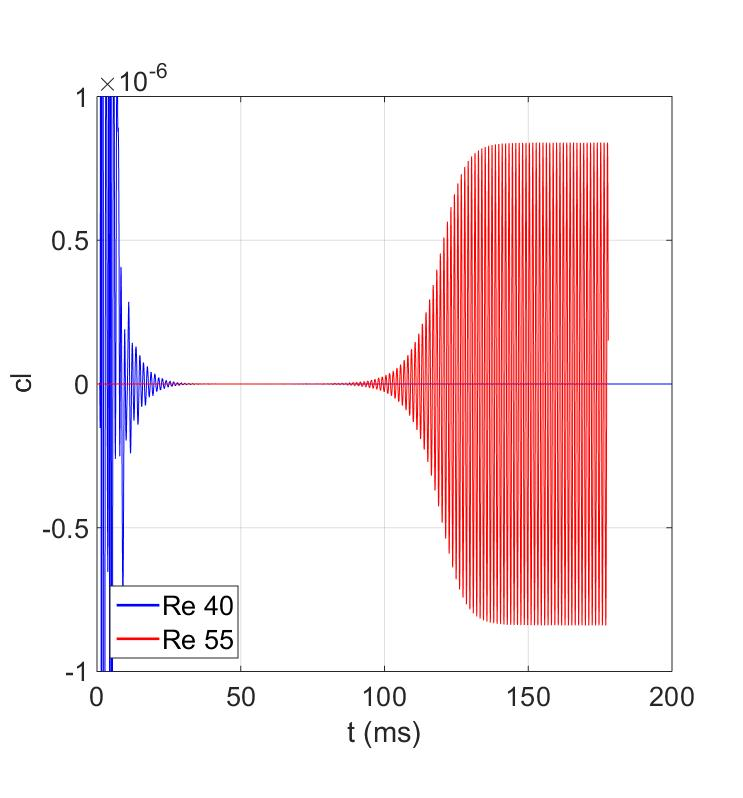
\includegraphics[width=0.3\textwidth]{pic/cl-linear.jpg}	
	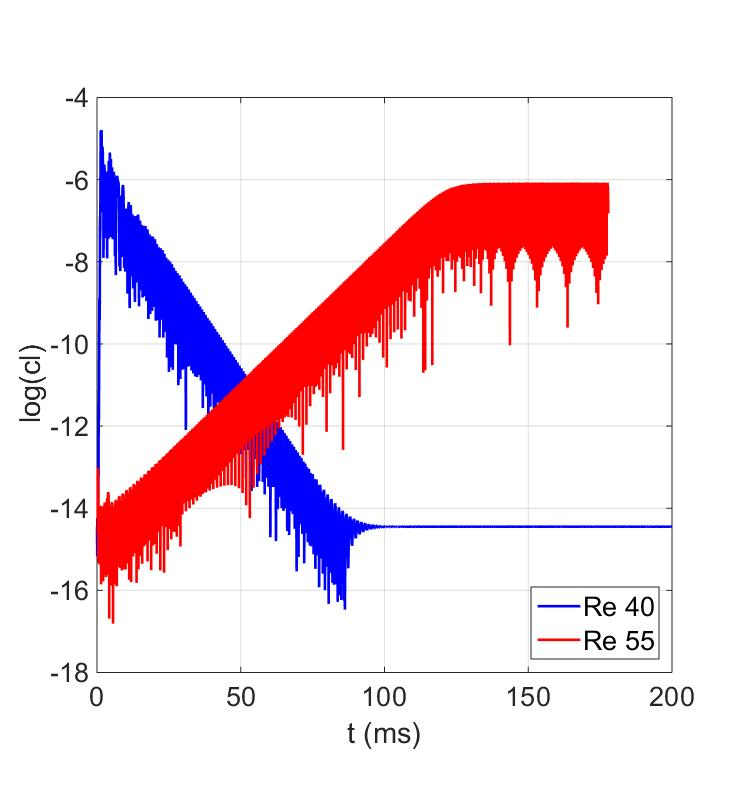
\includegraphics[width=0.3\textwidth]{pic/cl-log.jpg}
	\caption{Lift coeffient histogram for $Re=55$ and $Re=40$.}
	\label{fig:cyl-re40-re55-uns}
\end{figure}

\subsubsection{Eigenanalysis}
Eigenanalysis is performed for the steady state solution calculated
in NutsCFD. After converging the steady state solver to machine error ($tol=10^{-14}$),
the exact Jacobian matrix based on the 2nd-order spatial accuracy is calculated and
output to file. Arpack is used to computed a subset of the eigenvalues, with the aim of
finding the least stable mode.
To minimize the computational effort, 10 eigenvalues/vectors
are computed for matrices with different shifts of $0$, $i$, $2i$, $3i$, $4i$, $5i$. All the
eigenvalues, 60 in total and with some duplicated, are plotted
in Fig.~\ref{fig:cyl-re55-eigen-vs-uns}.
It can be seen that there is one eigenvalue that is on the right side of the imaginary axis,
indicating there is one unstable mode. In the meantime, from the time-domain simulation,
one can extract from the lift-coefficient signal that the flow is exponentially growing with
a growth rate of 0.123 and oscillating with a circular frequency of $4.94~rad/s$. This
value is plotted along with the spectrum and it can be seen that it overlaps with the
unstable eigenvalue from the eigenanalysis. 

\begin{figure}[htb]
	\centering   
	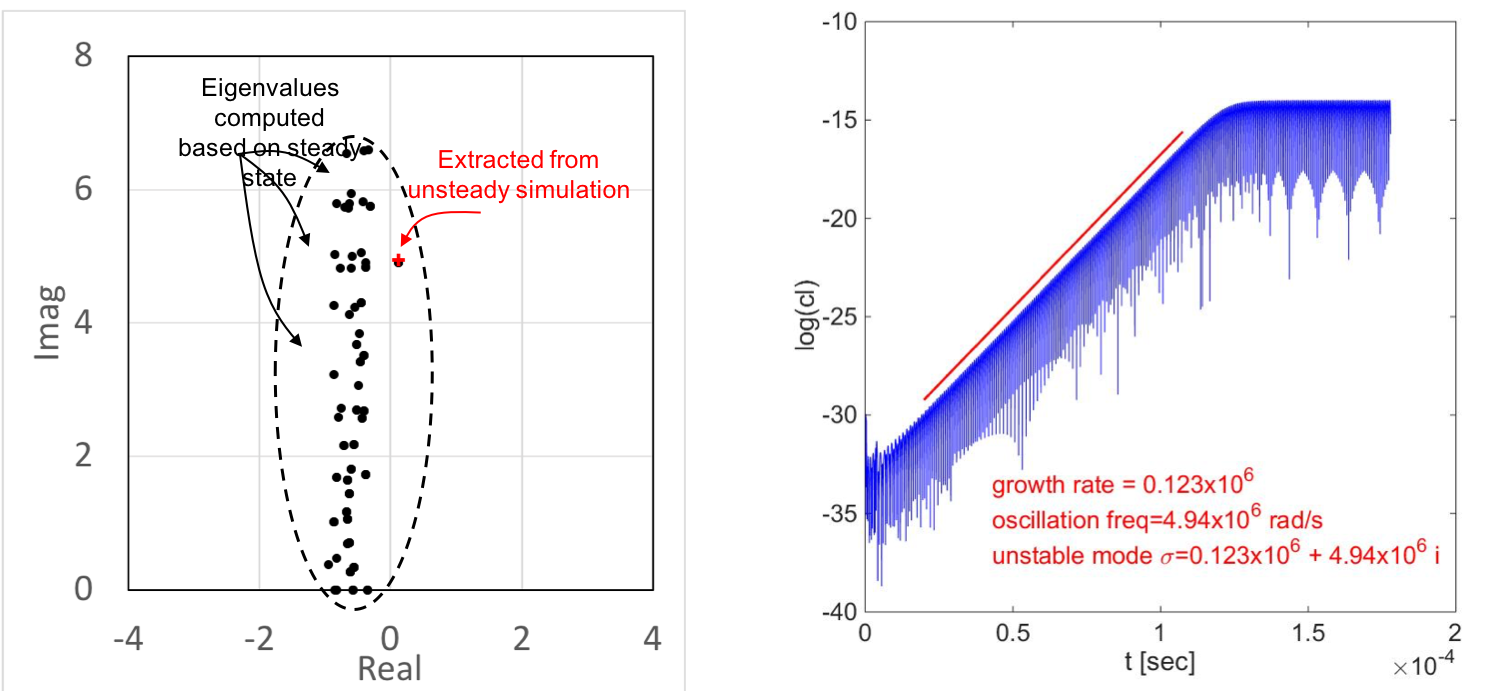
\includegraphics[width=0.6\textwidth]{pic/uns-vs-eigen.png}	
	\caption{Eigenspectrum from the steady state eigenvalue analysis
		compared with the linearly destabiling unsteady simulation for $Re=55$.}
	\label{fig:cyl-re55-eigen-vs-uns}
\end{figure}

The eigenanalysis not only generates the eigenvalues but also the eigenvectors
associated with each eigenvalue. For the unstable mode, the real part of the
density, x/y momentum and energy component of the unstable eigenvector
is shown in Fig.\ref{fig:cyl-re55-eigenmode}. Although not further explored
here, these eigenvectors will be useful for constructing reduced-order-models,
which can be used for rapid parameter study or fast time-domain responce.
\begin{figure}[htb]
	\centering   
	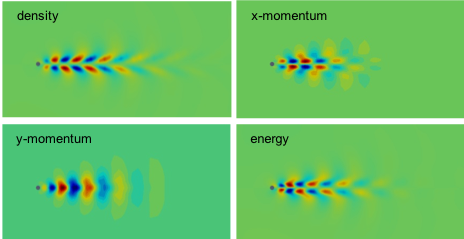
\includegraphics[width=0.6\textwidth]{pic/eigenmode-real.png}	
	\caption{Real part of the density, x/y momentum, energy components
		of the unstable eigenmode for $Re=55$.}
	\label{fig:cyl-re55-eigenmode}
\end{figure}

\subsubsection{Bifurcation tracking}
\begin{figure}[htb]
	\centering   
	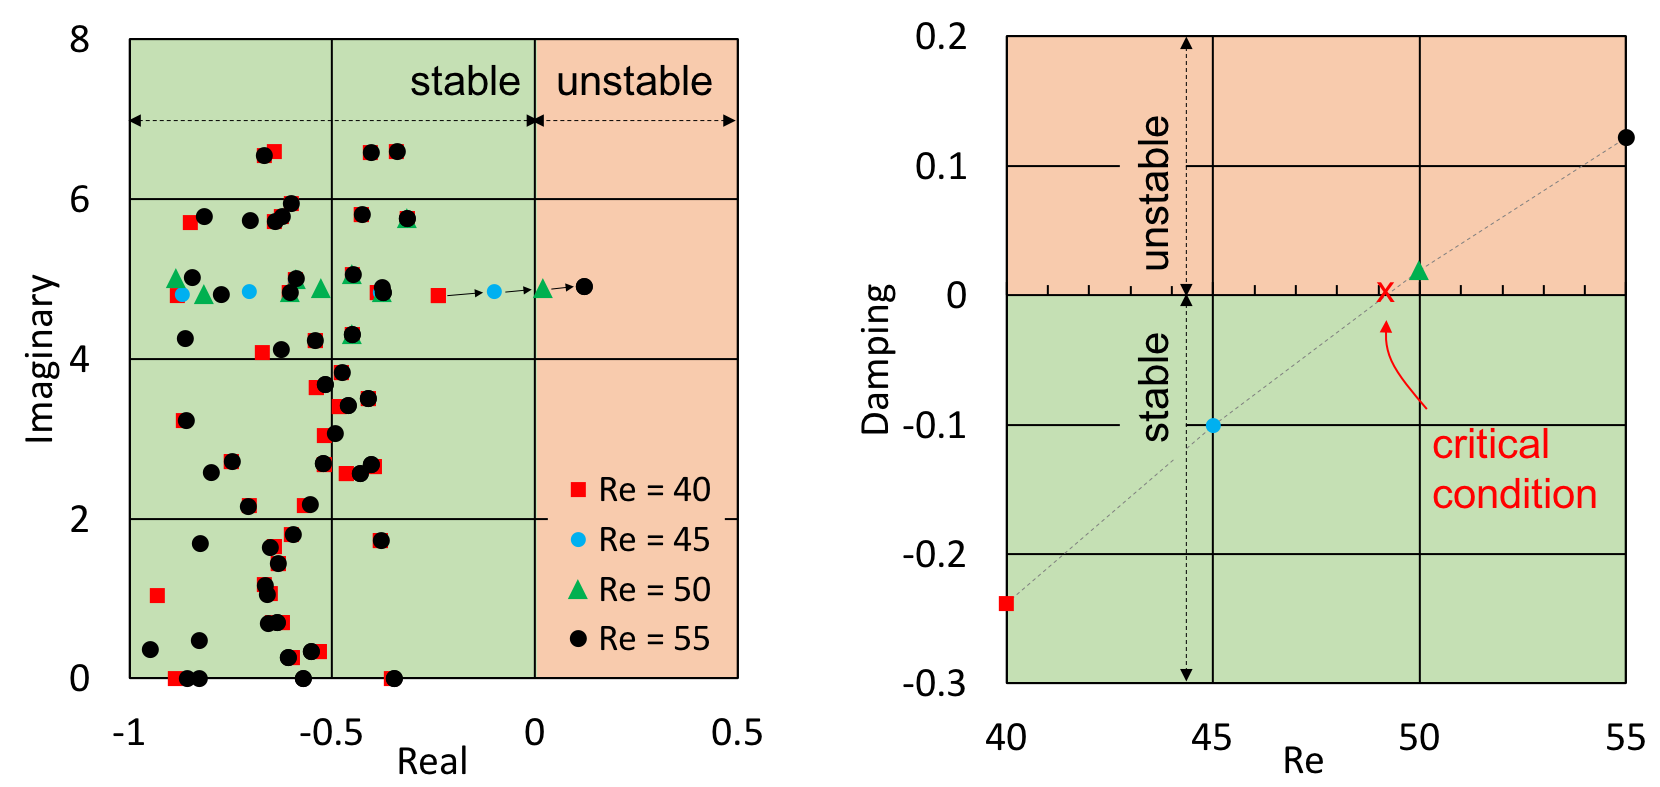
\includegraphics[width=0.7\textwidth]{pic/cylinder-bifurcation.png}	
	\caption{The spectra for $Re=40, 45, 50$ and $55$ (left) and the damping v.s. the Reynolds number (right).}
	\label{fig:cyl-bifur}
\end{figure}

The same procedure for computing the eigenvalues for $Re=55$ is applied to flows at $Re=40$, 45, and 50
to obtain their respective spectra, which is shown in Fig.~\ref{fig:cyl-bifur}. It can be seen that as the
bifurcation parameter $Re$ is increased from 40 to 55, one eigenmode becomes linear unstable. The
real part of this eigenvalue is plotted against $Re$ on the right in Fig.~\ref{fig:cyl-bifur}. It across the
imaginary axis at approximately $Re=49$, consistent with the experimental value of $Re_{crit}=47$.
Note that shown in the figure is only the upper half of the spectrum and the complex conjugate of
the destabilizing eigenvalue is thus not visualized. This is a classic Hopf bifurcation as the conjugate
complex eigenpair destabilizes simultaneously. However, it should be noted
that although linear stability analysis can predict the exact bifurcation, frequency predicted
based on the unstable eigenvalue beyond that
critical bifurcation parameter, $Re_{crit}$, should be used with care as it is different
from the vortex shedding frequency except very close to onset, for the laminar flow
around a long cylinder~\cite{barkley2006linear}. The implication on general cases
is yet to be explored in future work.

\subsection{Transonic flow for an isolated rotor row (quasi-3D analysis)}
NutsCFD is used to analyze the performance of the first
stage rotor (NASA Rotor 67) of a two stage transonic fan
designed and tested at the NASA Glenn center~\cite{strazisar1989laser}.
Its design pressure ratio is
1.63, at a mass flow rate of 33.25 kg/sec. 
The NASA Rotor 67 has 22 blades with tip radii of 25.7 cm
and 24.25 cm at the leading and trailing edge, respectively,
and a constant tip clearance of 1.0 mm. The hub to tip radius
ratio is 0.375 at the leading edge (TC = 0.6\% span) and 0.478
at the trailing edge (TC = 0.75\% span). The design rotational
speed is 16,043 RPM, and the tip leading edge speed is 429 m/s
with a tip relative Mach number of 1.38.

As a first step, the analysis is performed on the surface of
revolution taken at approximately 50\% of the blade height.
The three-dimensional mesh has one cell in the radial direction
and the subsequent analysis is thus a quasi-3D one.

\subsubsection{Steady state calculation}
Steady state analysis is performed for both
the single-passage and whole-annulus
configurations. In order to obtain the steady state
solutions for the whole annulus, which presumably
is identical for each blade passage, we first compute
the steady state solution for one passage with
rotatioal periodicity, and then copy the solution
to the whoe annulus using rotational transformation.
Due to the slight difference in discretization, a fully-converged
flow solution for one-passage produces a finite residual
after it is copied to the whole annulus, and therefore a few
extra iterations are required on the whole-annulus mesh to
fully converge the flow to machine error.
The pressure ratio and efficiency are shown
in Fig.~\ref{fig:r67-performance}
which is produced by incrementally raising the back pressure
from the inlet total condition. It can be seen that there is a small
difference (mainly efficiency) between the single-passage and
whole-annulus results, which is due to the minor discrepancy
of the spatial discretization at the periodic boundaries for single
passage calculation.
The flow solution using the whole annulus is shown in Fig.~\ref{fig:r67-flow}.
No mesh convergence study has been performed.


\begin{figure}[htb]
	\centering   
	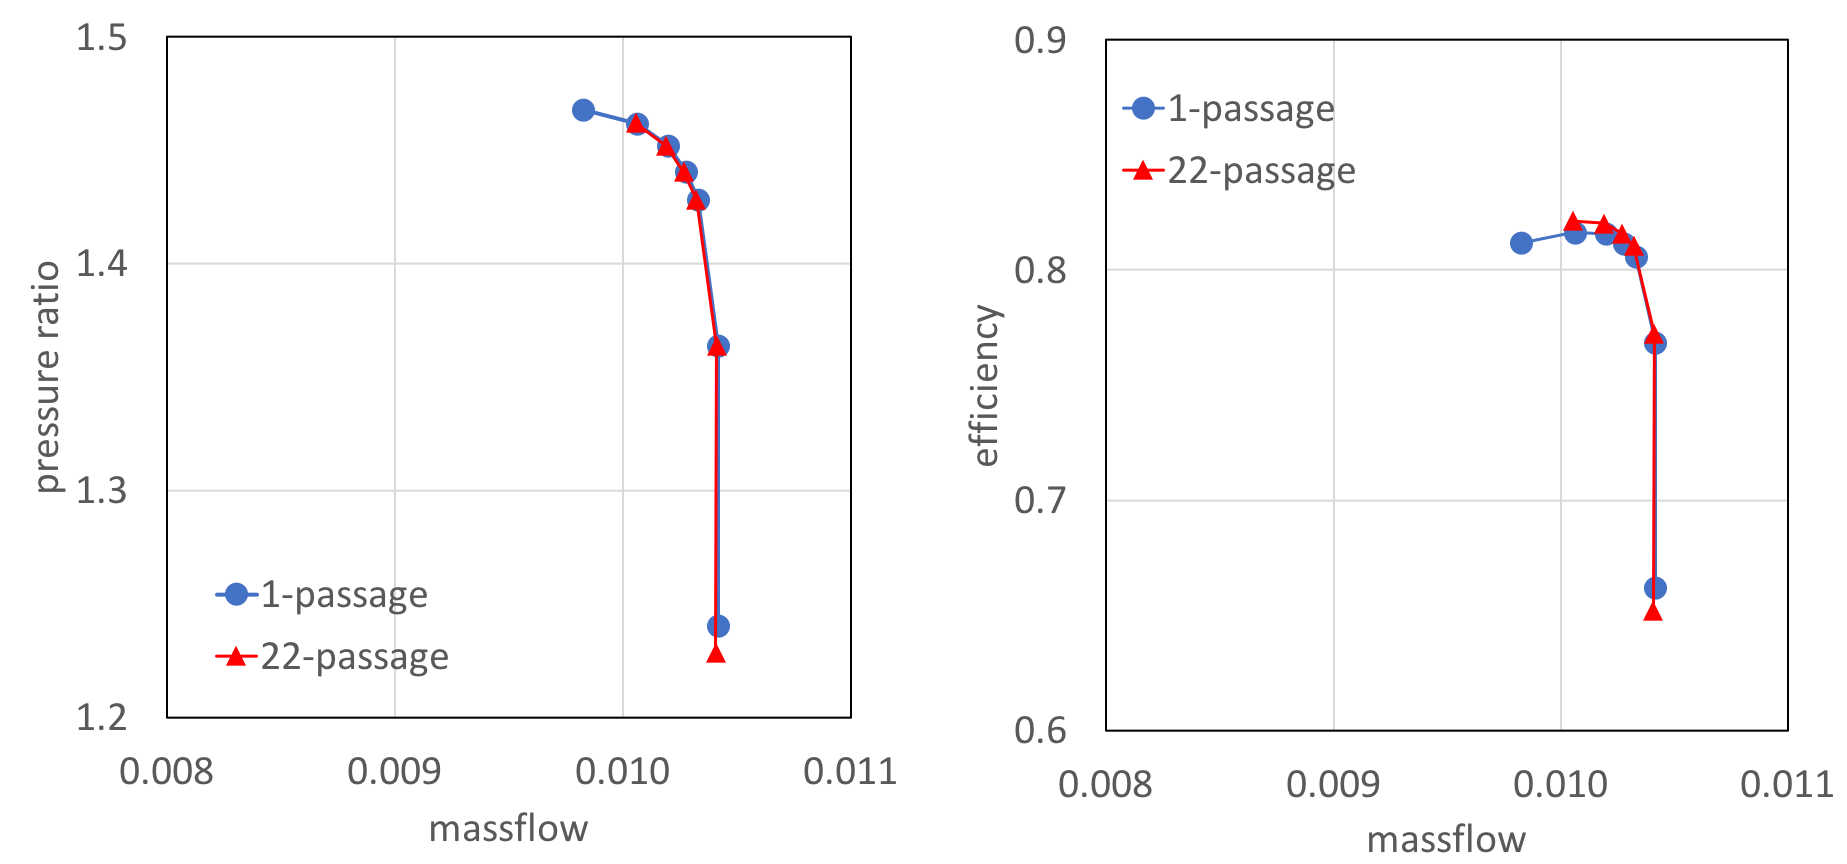
\includegraphics[width=0.6\textwidth]{pic/rotor67-performance.png}
	\caption{Q3D performance for rotor67 at 50\% blade height with either
		single passage or whole annulus.}
	\label{fig:r67-performance}
\end{figure}



\begin{figure}[htb]
	\centering   
	%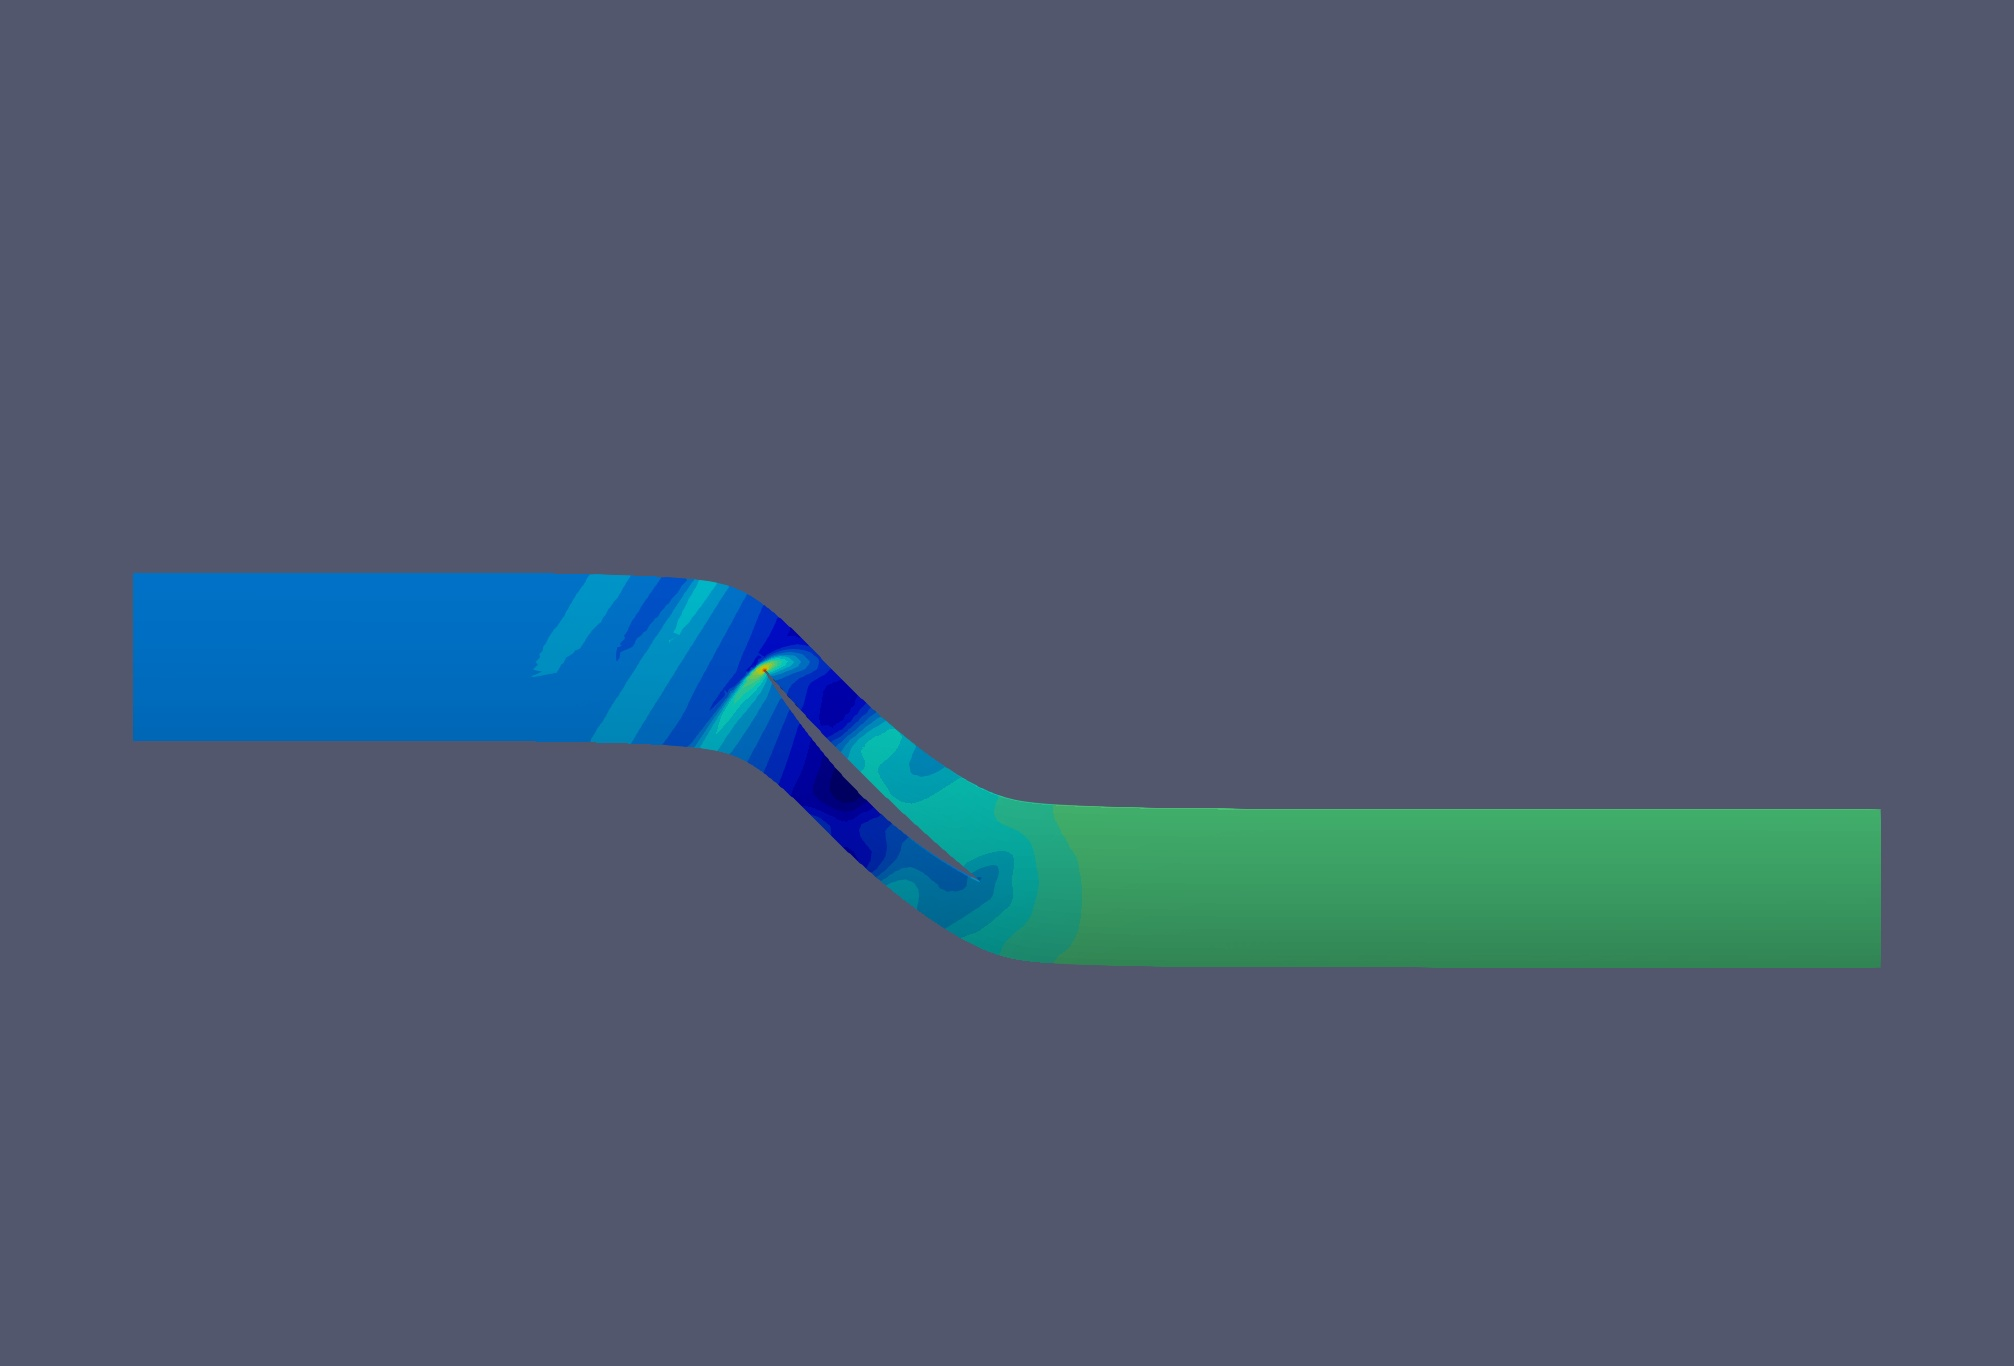
\includegraphics[width=0.35\textwidth]{pic/pressure-1passage.jpeg}
	%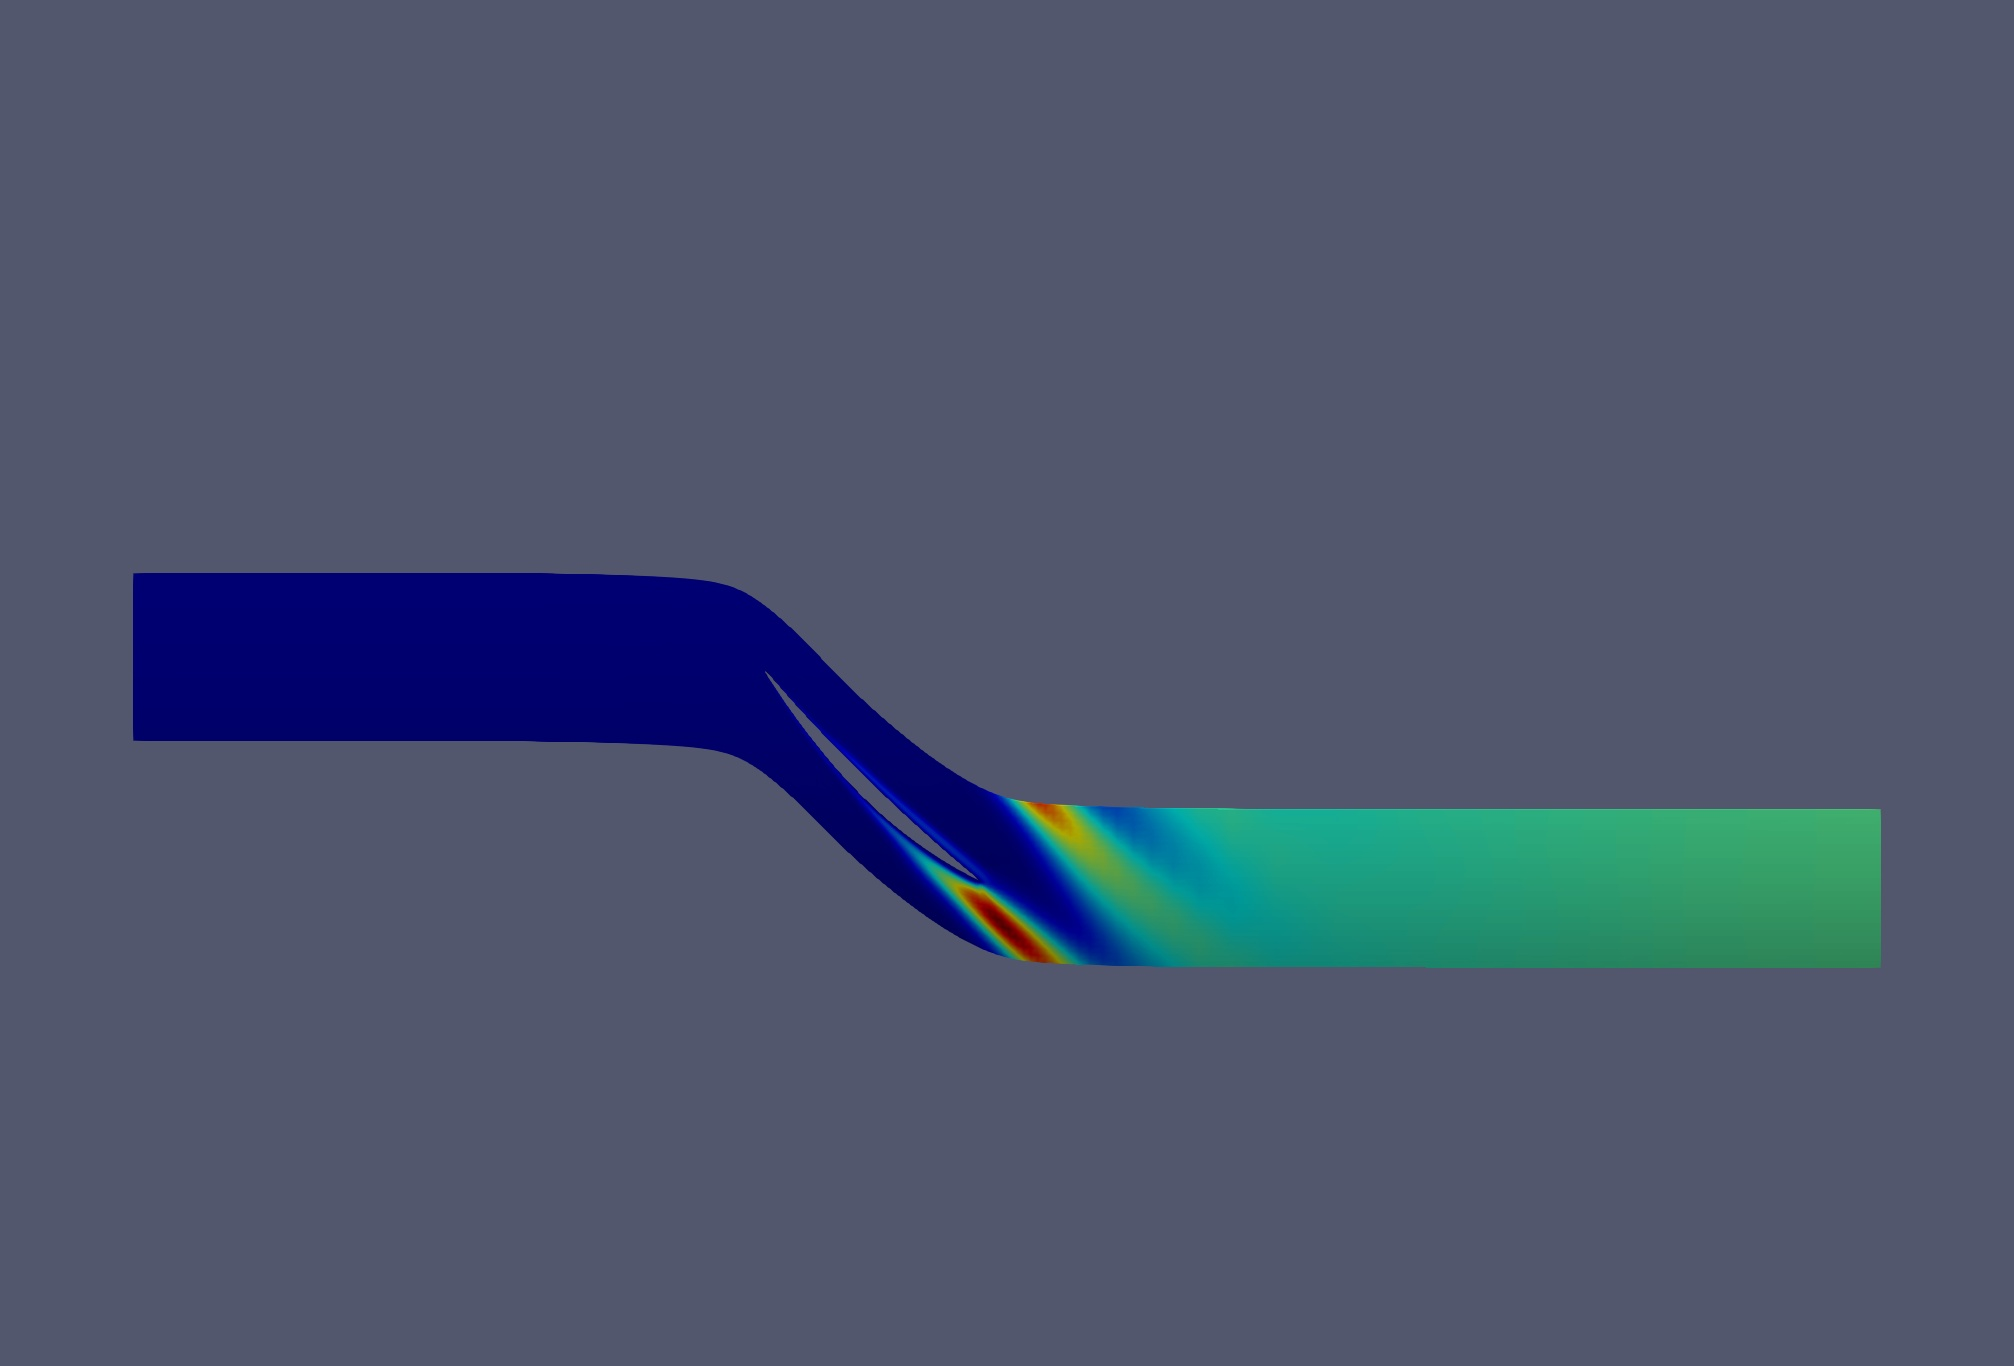
\includegraphics[width=0.35\textwidth]{pic/sa-1passage.jpeg}\\    
	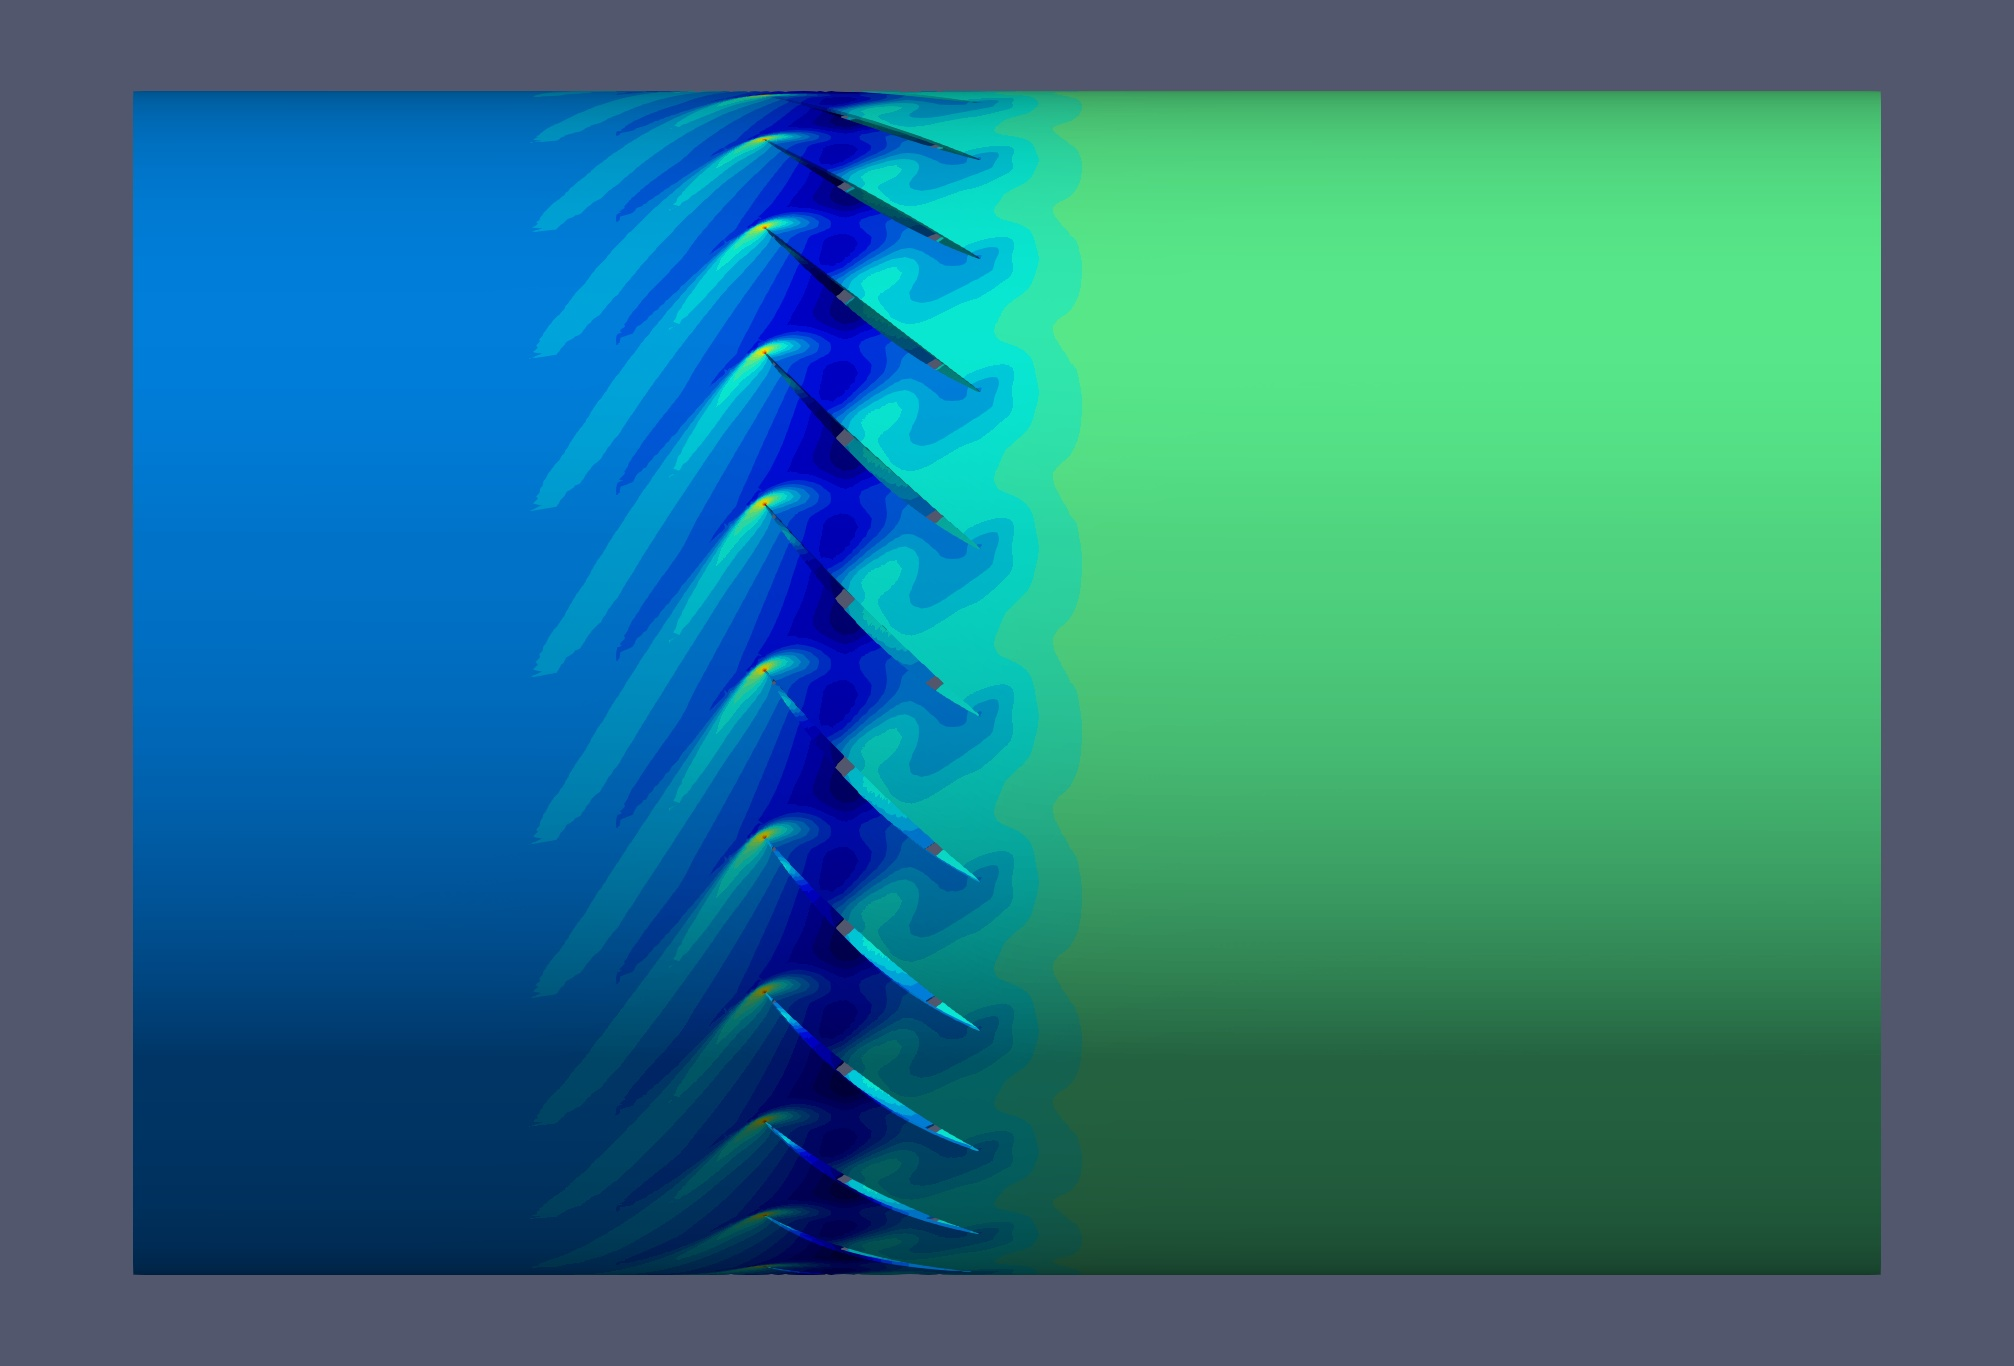
\includegraphics[width=0.35\textwidth]{pic/pressure-22passage.jpeg}
	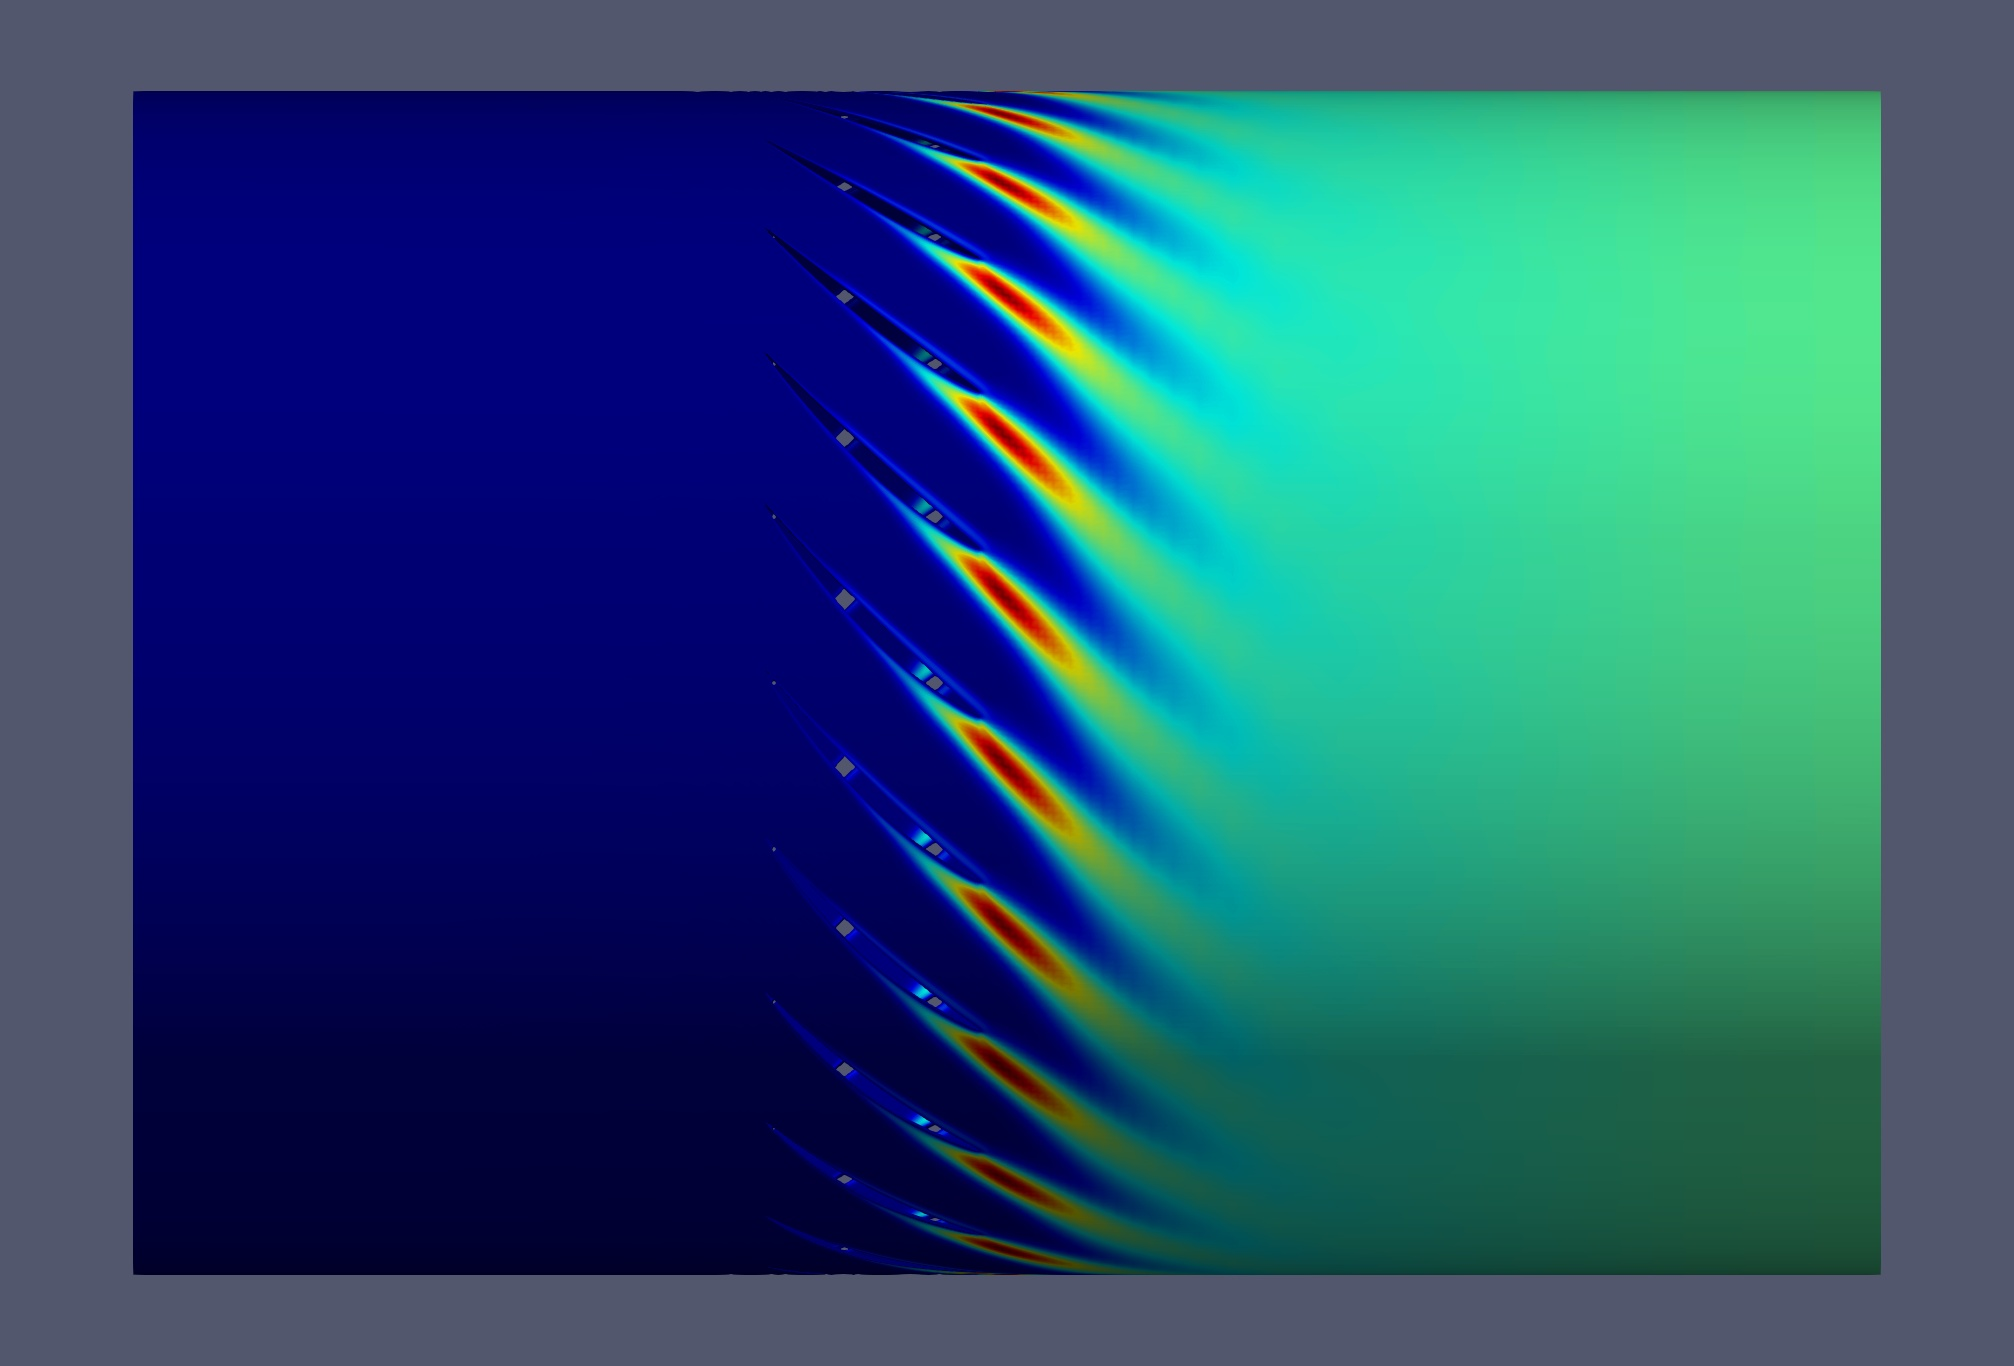
\includegraphics[width=0.35\textwidth]{pic/sa-22passage.jpeg}
	\caption{Pressure (left) and SA variable (right) contours for
	whole-annulus calculations.}
	\label{fig:r67-flow}
\end{figure}

\subsubsection{Eigenanalysis}

For each whole-annulus steady state solution, eigenanalysis
is performed using the Jacobian matrix output from the NutsCFD solver
once the steady state calculation has fully converged.
Since the rotational speed for the rotor is 16043 RPM, the Jacobian
matrix is scaled by a factor of $1/(2\pi \times 16043 / 60)\approx 1/1680$,
so that all frequencies involved in this computation is normalized by the
shaft angular frequency. This is done due to the pre-knowledge that
rotating stall cells move with a speed of the same order of magnitude
as the shaft speed.

One the flow has fully converged, the left most point on the whole-annulus
performance curve is used for eigenanalysis.
Shown in Fig.~\ref{fig:r67-eigenvalue-18kpa} is a subset of the eigenvalues
that are near the imaginary axis, which presumally are most likely to
be unstable. ARPACK is used with various imaginery shifts to compute
interior eigenvalues. The ones that are suspecious of crossing the
imaginery axis are shown. A zoomed view of the eigenvalues reveals
that there are a total of five that have positive real parts, i.e., unstable.
A single-mode instability is not found for in case most likely because
the flow condition chosen is one that is deep into the linearly unstable
region and a bifurcation point should be searched for at a higher flow-rate
condition. Nevertheless, in the work, we restrict outselves to the analysis
of this single condition and a thorough exploration of the whole picture will
be conducted in our future work.


\begin{figure}[htb]
	\centering   
%	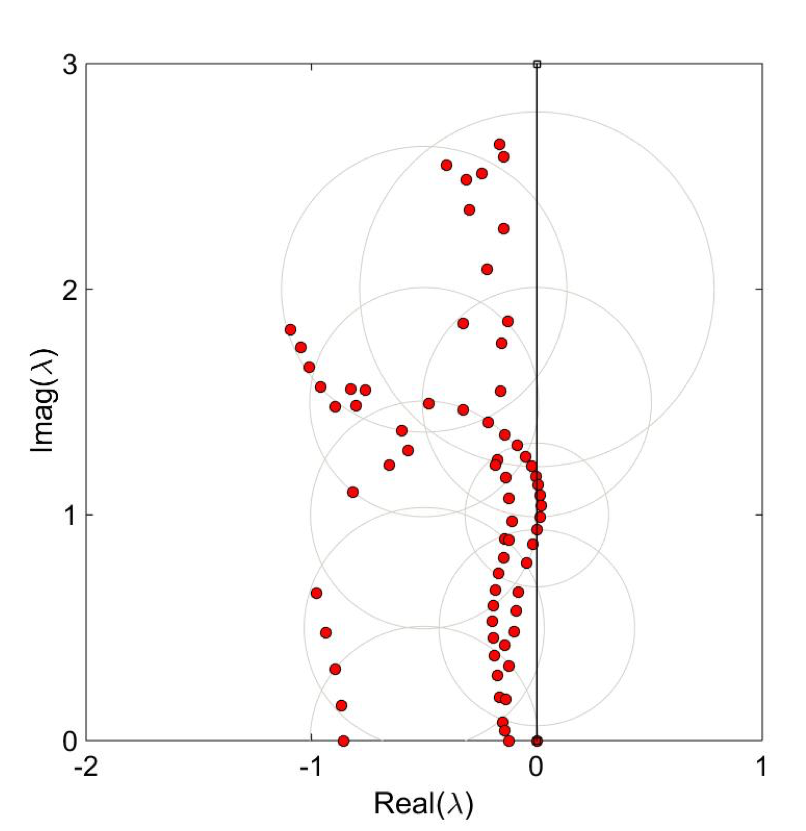
\includegraphics[width=.4\textwidth]{pic/eigenvalue-18kpa.png}
	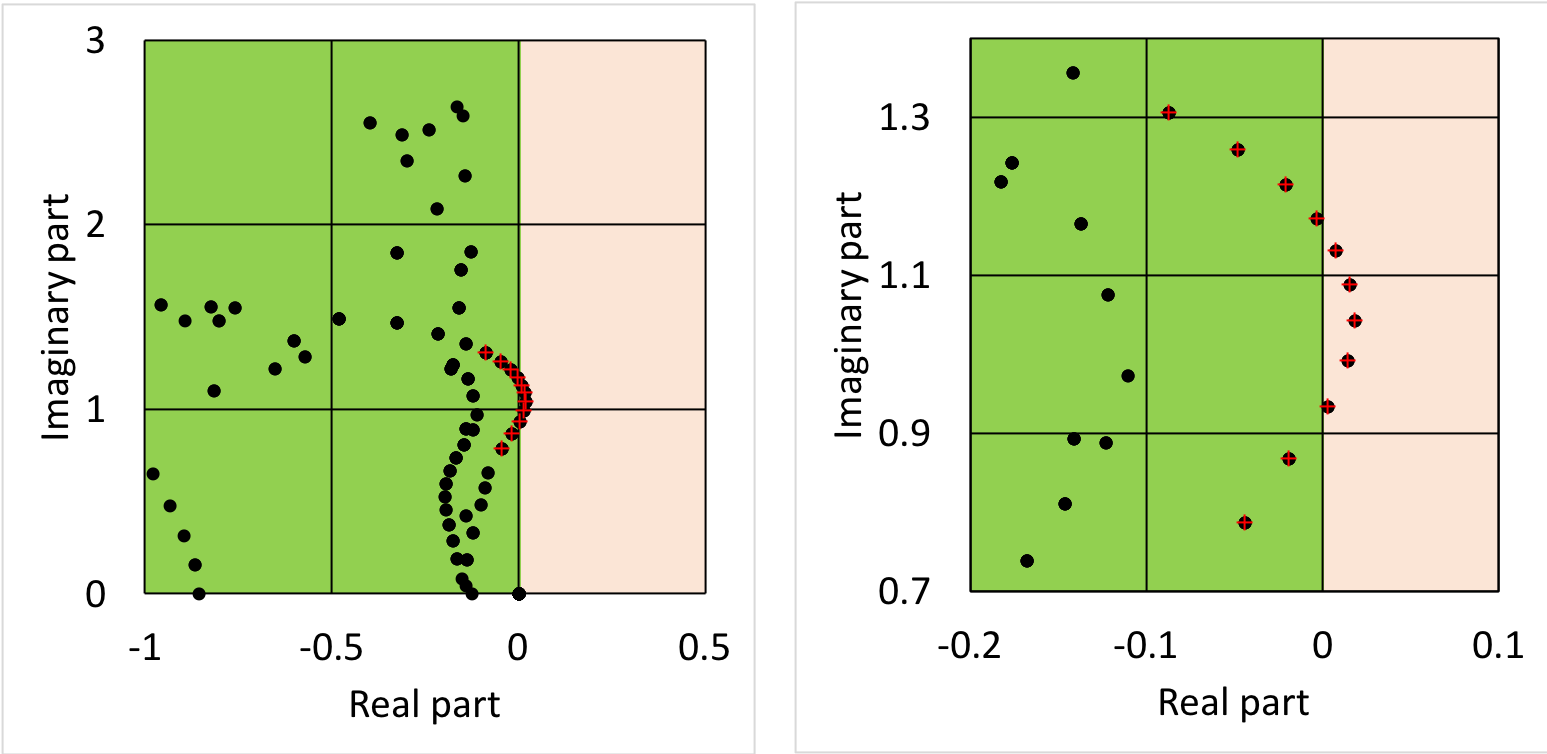
\includegraphics[width=.7\textwidth]{pic/rotor67-18kpa-spectrum.png}	
	\caption{Spectrum for stall condition.}
	\label{fig:r67-eigenvalue-18kpa}
\end{figure}

The unstable eigenvector with the smallest imaginary part (lowest point amont the
five unstable eigenvalues) is visualized in Fig.~\ref{fig:r67-eigenvector-18kpa} with
both the real and imaginary parts. The circumferential shock
oscillation can be seen. To analyze the spatial modes, data along
the intersecting curve is taken (marked at the red line in
Fig.~\ref{fig:r67-eigenvector-18kpa}). This is done for
each of the 11 modes (marked with red cross in Fig.~\ref{fig:r67-eigenvalue-18kpa}). It is clear from the spatial Fouriour analysis
that each eigenvector corresponds to a rotating pattern with a different
nodal diameter, which increases from 1 to 11 monotonically from the lowest
to the highest eigenvalues.

\begin{figure}[htb]
	\centering   
	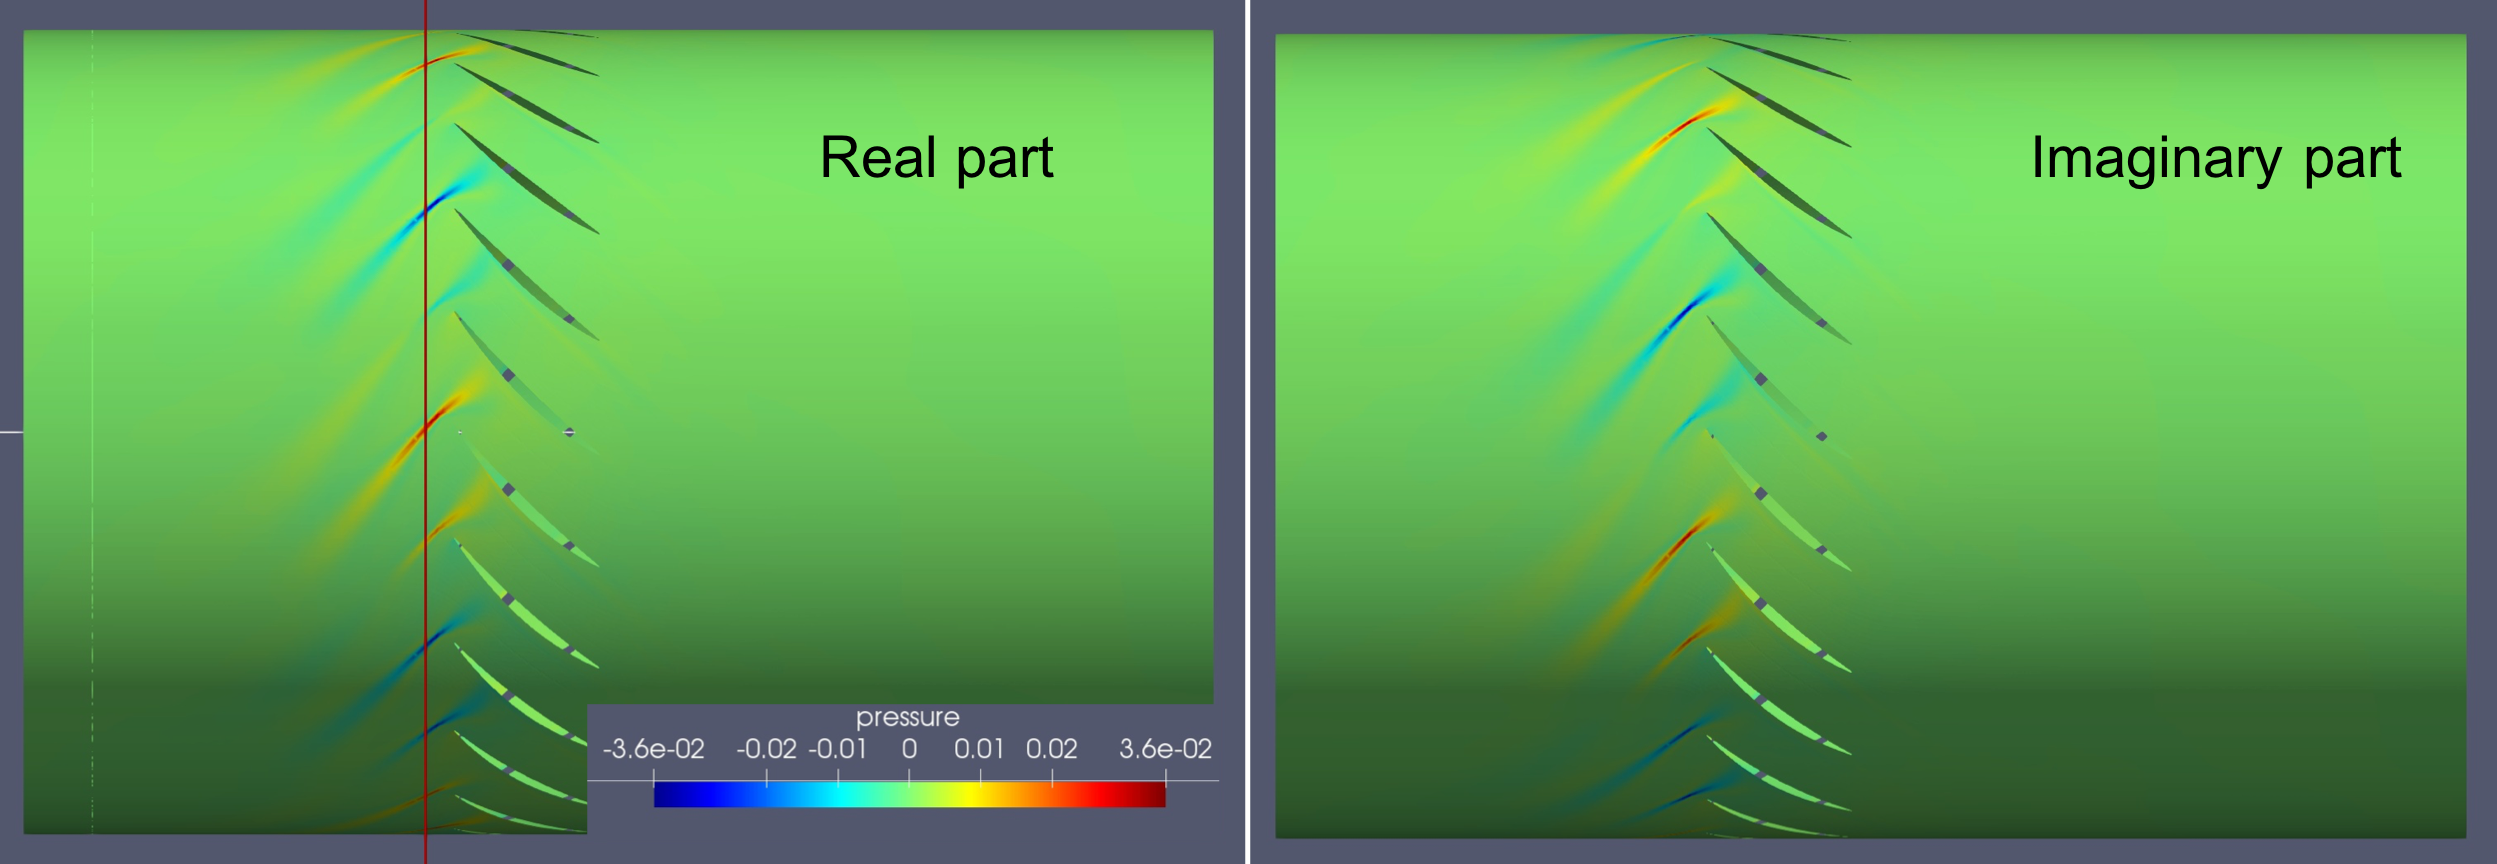
\includegraphics[width=.6\textwidth]{pic/mode-with-nd5.png}
	\caption{Eigenvector 5 visualized using the real and imaginary parts
		of energy component}
	\label{fig:r67-eigenvector-18kpa}
\end{figure}

%\begin{figure}[htb]
%	\centering   
%	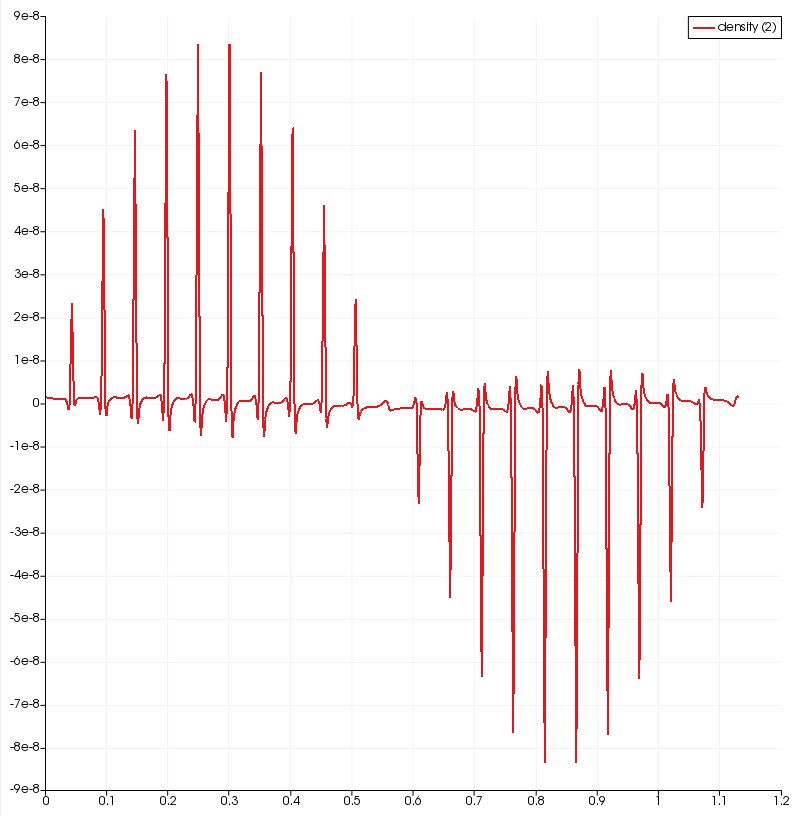
\includegraphics[width=.2\textwidth]{pic/mode1-nd1.jpg}~~~~
%	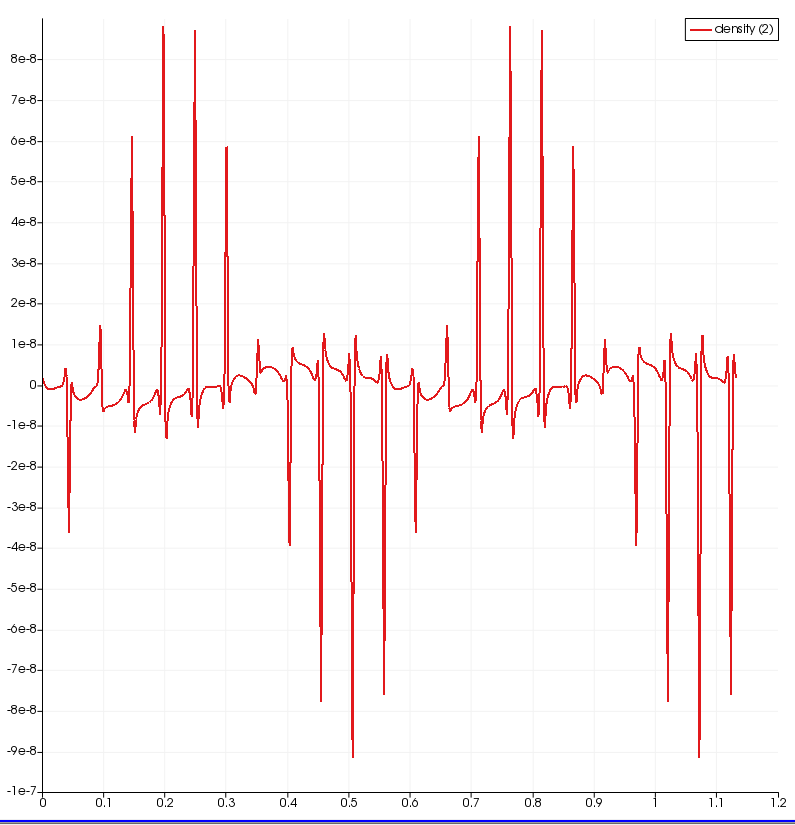
\includegraphics[width=.2\textwidth]{pic/mode2-nd2.jpg}~~~~
%	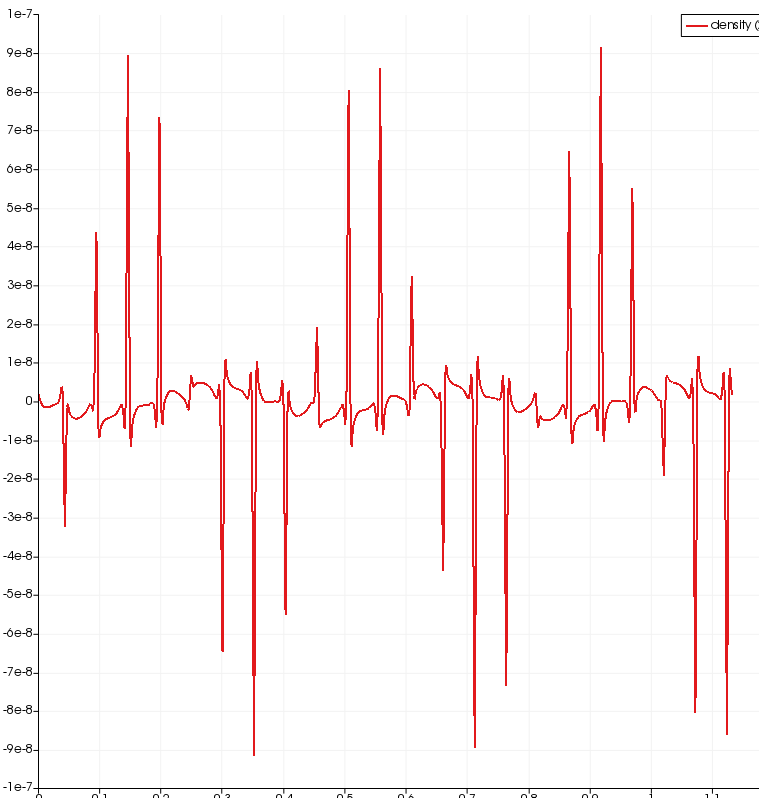
\includegraphics[width=.2\textwidth]{pic/mode3-nd3.jpg}~~~~
%	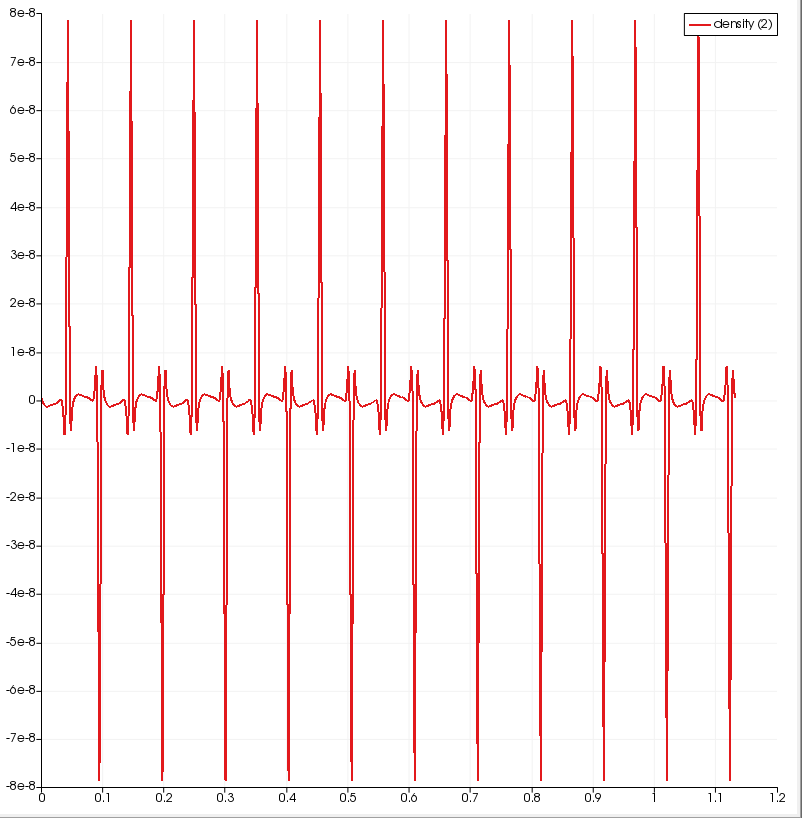
\includegraphics[width=.2\textwidth]{pic/mode11-nd11.jpg}			
%	\caption{The circumferential distribution for the real part of the
%	pressure component of the 1st, 2nd, 3rd and 11th eigenvectors.}
%	\label{fig:r67-data-circumferential}
%\end{figure}

A more involved data processing reveals that the perturbation pattern,
for every eigenvector, is a travelling wave that rotates in the opposite
direction of the motion of the rotor (in the relative frame), and with a speed a fraction of the
shaft rotating speed. This relative rotating speed can be
calculated using the imaginary of the eigenvalue and the nodal diameter
of the perturbation pattern as $\dfrac{\text{Imag}(\lambda)}{\omega_{shaft}} \dfrac{1}{ND}$.
%In experiments, instrumentation for detecting rotating instability is usually
%sensors installed on the stationary casing and the speed of the rotating
%cells is also measured in the absolute reference frame.
In the absolute reference frame, the cell rotating speed (normalized
with shaft angular frequency) is calculated as
\begin{equation}\label{cellrotspd}
U_{cellRotating}= 1-\dfrac{\text{Imag}(\lambda)}{\omega_{shaft}} \dfrac{1}{ND}.
\end{equation}
Applying this formula to each of the 11 eigenmodes leads to the
correlation between the nodal diameter and the perturbation rotating speed, as shown in Fig.~\ref{fig:r67-eigenvector-18kpa}. Note that we use the terminology 'cell rotating speed'
to be consistent with the language used by experimentalists when they describe
the rotating cells. In fact, what is meant in the current context is actually
`rotating speed of the perturbation pattern'.
Although it is well-known that the conclusions drawn from a global linear
stability analysis can not represent the behavior of a saturated limit cycle
which is highly nonlinear, it seems that the characteristics of the
rotating perturbation,
in terms of nodal diameter and rotating speed, is qualitatively representative
of rotating cells observed experimentally. However, questions such as which eigenmode
should destabilizes first, and how does the inlet distortion and blade-row interaction in
multirow configuration affect the conclusion, remain to be answered.

\begin{figure}[htb]
	\centering   
{\tiny }	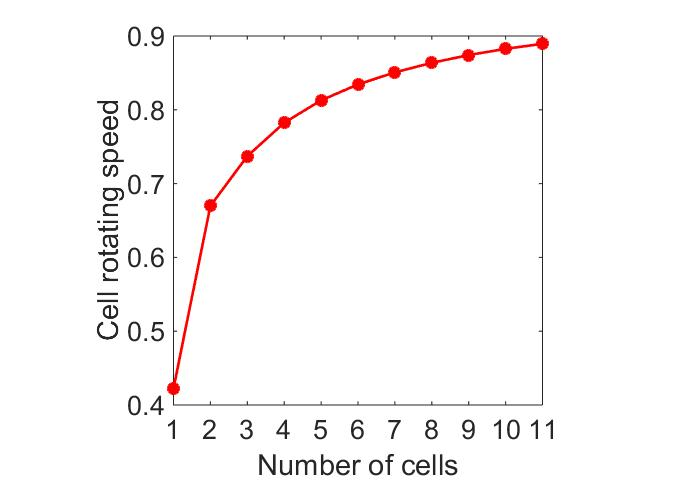
\includegraphics[width=.4\textwidth]{pic/speed-vs-nd.jpg}
	\caption{The cell rotating speed v.s. the number of cells (nodal diameter of the perturbation pattern).}
	\label{fig:r67-eigenvector-18kpa}
\end{figure}

\section{Conclusion}
\label{conclusion}

Rotating flow instability at near stall condition for an annular compressor cascade is studied using the eigenanalysis approach and the destabilizing eigenmodes are computed and
analyzed to shed insight on the rotating stall phenomenon. 
This is the first time a full-order gloabl linear stability analysis based on
the three dimensional RANS equations is performed to study the destabilising
mechanism of such turbomachinery flow phenomenon.

Specifically, a stable nonlinear flow solver based on the matrix-forming Newton--Krylov
approach is used to compute the steady state flow solution at near stall (possibly
post-stall) condition and the readily available exact Jacobian matrix is then used
for eigenvalue anlaysis. The eigenanalysis is performed to compute a subset of
the eigenvalues that are near the imaginary axis, with the implicit-restarted
Arnoldi method implemented in the ARPACK library. The shift-and-invert
approach is used to obtain the least unstable eigenvalues.

The methodology is first applied to the classic case of a laminar flow around
a 2D circular cylidner. By perturbing the system parameter $Re$, Hopf
bifurcation is identified which is responsible for the inception of the laminar
vortex shedding. The frequency and linear growth ratio from the eigenanalysis
agree well with time-dependent simulation during the linear growth regime.

The same procedure is then applied to the a quasi-3d compressor rotor.
Analysis shows the existance of a complete set of spatial modes that have
different nodal diameters and
rotating speeds. These analysis results provide a solid foundation for the
explanation of various observations in experiments regarding
rotating flow instabilities. It is revealed that the multiple modes with
different nodal diameters coexist, as the inherent property of the
physical system, and it can be hypothesized that the reason for
different observed stall cell patterns is due to one particular mode being
excited to finite amplitute first by external disturbance.
Further more, by processing the spatial modes and the imaginary
part of the eigenvalues, rotating speeds of the perturbation patterns
can be calculated and are found to qualitatively agree with the various
experimentally observed values for rotating stall cells.

The preliminary results presented in this paper represent our first
attempt to use eigenanalysis based on RANS equations to study
the rotating flow instability phenomenon in turbomachinary flows.
The results are promising in that it shows the eigenanalysis method
is feasible for practical cases and the eigenvectors do capture some
of the key featuers of the flow instability investigated. However, more in-depth
study is needed to investigate the bifurcation process for the quasi-3D
case, and further investigation into three-dimensional cases will be
carried out in our future work.

%The results also indicate that the incipent rotating stall is dominated by the
%dynamics of a single complex-conjugate pair of unstable eigenmodes.
%This provides a clarification of the currently widely spreaded
%explainations regarding the origin of the rotating stall. In line with the
%classical explaination of the modal wave instability route to rotating stall,
%the full-order CFD analysis in this work confirms this, but provides a much
%better understanding of the detailed flow physics when such instability
%occurs.


\section*{Acknowledgements}
This work received support by the National Natural
Science Foundation of China (Grant No.~51790512).


\bibliography{xu}

\end{document}
